\documentclass[11pt,compress,t,notes=noshow, xcolor=table]{beamer}

\input{../../style/preamble}
\input{../../latex-math/basic-math}
\input{../../latex-math/basic-ml}

\title{Applied Machine Learning}
% \author{LMU}
%\institute{\href{https://compstat-lmu.github.io/lecture_iml/}{compstat-lmu.github.io/lecture\_iml}}
\date{}

\setbeamersize{text margin left=0.3cm,text margin right=0.3cm}


\begin{document}

\titlemeta{
PLACEHOLDER
}{
Feature Engineering 2 - Feature Selection
}{
figure_man/empty
}{
	%\item Imputation
    \item Reasons for Feature Selection
    \item Types of Feature Selection
}


\section{Recap}

\begin{frame}{What is feature engineering?}
Feature engineering is on the intersection of \textbf{data cleaning}, \textbf{feature
creation} and \textbf{feature selection}.
\vfill
The goal is to solve common difficulties in data science projects, like
\vfill
\begin{itemize}
    \item skewed/weird feature distributions,
    \item (high cardinality) categorical features,
    \item functional (temporal) features,
    \item missing observations,
    \item high dimensional data,
    \item ...
\end{itemize}
\vfill
and improve model performance (or make the data readable by the model in the first place).
\end{frame}

\begin{frame}{Train-Test Leakage}
% This is so important, that I will just repeat this again!
% \includepdf[pages={2},trim=0 20 0 50,clip,width=400pt,offset=-60pt 10pt,pagecommand={}]{../05_feature-preproc/pdf_chapters/slides_leakage.pdf}
\begin{center}
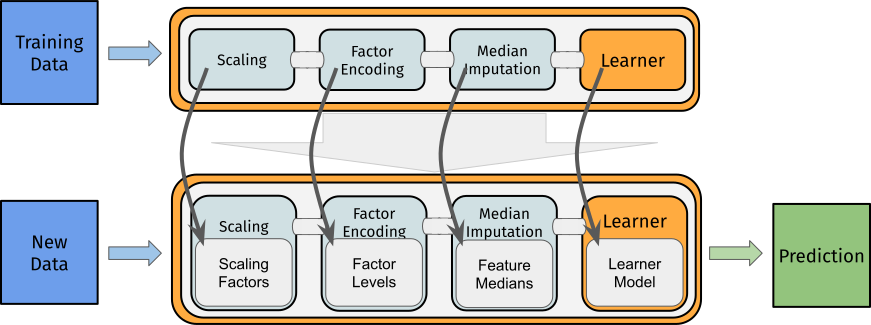
\includegraphics[width=\textwidth]{figure_man/pipe_action.png}
\end{center}

\end{frame}



\begin{frame}{Types of Feature Engineering (so far)}
\begin{itemize}
    \item numerical encoding of categorical features
    \item feature transformations
    \item imputation
\end{itemize}
\end{frame}

% slides\06_adv-feature-preproc-selection\sl\slides-fs-introduction.pdf
\section{Feature Selection}

\begin{vbframe}{Motivation}
\begin{itemize}
\setlength{\itemsep}{0.8em}
    \item Naive view:
    \begin{itemize}
        \item More features $\rightarrow$ more information $\rightarrow$ discriminant power $\uparrow$
        \item Model is not harmed by irrelevant features since their parameters can simply be estimated as 0.
    \end{itemize}
    %\item In practice there are many reasons why this is not the case!
    \item In practice, irrelevant and redundant features can \enquote{confuse} learners (see \textbf{curse of dimensionality}) and worsen performance.
    \item Example: In linear regression, $R^2$ is monotonically increasing in $p$, but adding irrelevant features leads to overfitting (capturing noise). %instead of underlying relationship.
\end{itemize}

\begin{center}
    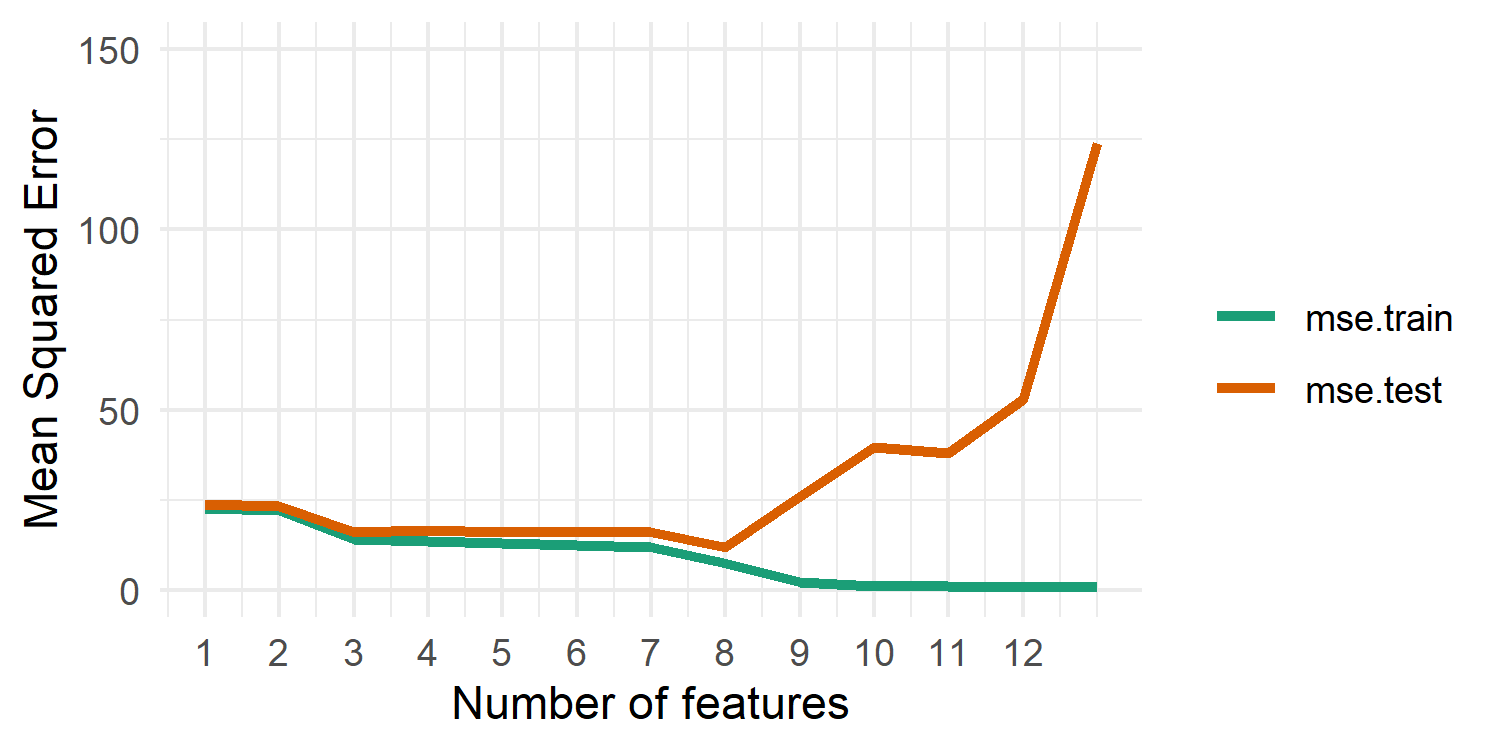
\includegraphics[width = 0.5\textwidth]{sl/feature-selection/figure/avoid_overfitting_02.png}\\
\end{center}

\framebreak

\begin{itemize}
\setlength{\itemsep}{1.0em}
    \item In high-dimensional data sets, we often have prior information that many features are either irrelevant %or redundant 
    or of low quality
    \item Having redundant features can cost something during prediction %cost something 
    (money or time)
    %\item Training data are limited.
    %\item Computational resources are limited.
    \item Many models require $n > p$ data. Thus, we either need to
    %\item Thus, we either need
    \begin{itemize}
    \item adapt models to high-dimensional data (e.g., regularization)
    \item design entirely new procedures for $p>n$ data
    \item use filter preprocessing methods from this lecture
    \end{itemize}
\end{itemize}
\end{vbframe}

\begin{vbframe}{Size of datasets}
Many new forms of technical measurements and connected data leads to availability of extremely high-dimensional data sets.

\vspace{0.5cm}
\begin{itemize}
\setlength{\itemsep}{1.2em}
    \item \textbf{Classical setting}: Up to around $10^2$ features, feature selection might be relevant, but benefits often negligible.
    \item \textbf{Datasets of medium to high dimensionality}:
    At around $10^2$ to $10^3$ features, classical approaches can still work well, while principled feature selection helps in many cases.
    \item \textbf{High-dimensional data}: $10^3$ to $10^9$ or more features.
    Examples: micro-array / gene expression data and text categorization (bag-of-words features).
    If we also have few observations, scenario is called $p \gg n$.
\end{itemize}

\end{vbframe}

\begin{vbframe}{Feature selection vs. extraction}

\begin{columns}
    %Both graphs taken out from Tim Conrad's presentation for Novisad (see cim2/external_material/tim_conrad_novisad)

    \column{0.49\textwidth}
    %\textbf{Feature selection}

    \medskip

    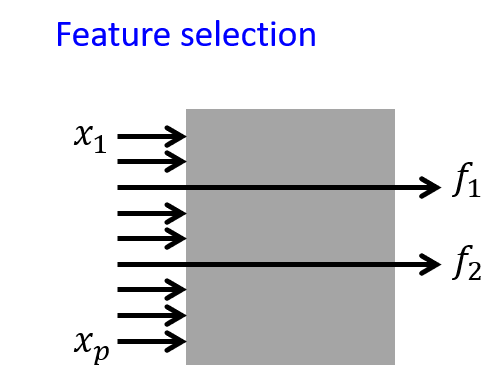
\includegraphics{sl/feature-selection/figure_man/feature_selection.png}

    \smallskip

    \begin{itemize}
    \item Creates a subset of original features $\xv$ by selecting $\tilde{p} < p$ features $\bm{f}$.
    %\item Selected features are subset of $\xv$.
    \item Retains information on selected individual features.
    \end{itemize}

    \column{0.49\textwidth}
    %\textbf{Feature extraction}

    \medskip

    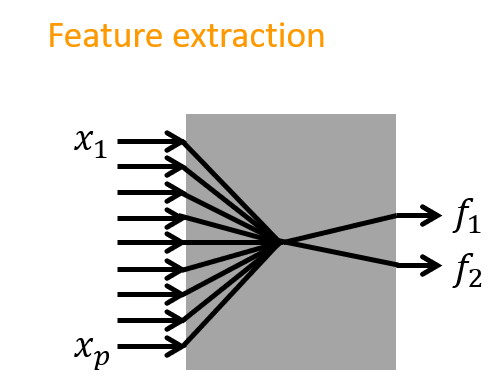
\includegraphics{sl/feature-selection/figure_man/feature_extraction.png}

    \smallskip

    \begin{itemize}
    \item Maps $p$ features in $\xv$ to $\tilde{p}$ extracted features $\bm{f}$.
    %\item Forms linear or nonlinear combinations of the original features.
    \item Info on individual features can be lost through (non-)linear combination.
    \end{itemize}

\end{columns}

\end{vbframe}

\begin{frame}{Reasons for feature selection}
\begin{itemize}
    % All from https://mlr3book.mlr-org.com/chapters/chapter6/feature_selection.html#sec-fs-filter
    \item improved predictive performance, since we reduce overfitting on irrelevant features,
    \item robust models that do not rely on noisy features,
    \item simpler models that are easier to interpret,
    \item faster model fitting, e.g. for model updates,
    \item faster prediction, and
    \item no need to collect potentially expensive features.
\end{itemize}
\end{frame}

\begin{frame}{Goals of feature selection}
% Source: https://link.springer.com/article/10.1007/s10618-020-00731-7
\vfill
\textbf{Single Feature Selection Problem:} identifying a minimal-size subset of the variables that is optimally predictive for an outcome variable T of interest.

%\vspace{1cm}
\vfill

% For this lecture the multiple feature selection problem is not relevant, but it is important that you have heard about it
\textbf{Multiple Feature Selection Problem:} Let $\mathcal{S}$ be the solution to the single feature selection problem (called the reference solution). The solution $\mathcal{M}$ to the multiple feature selection problem consists of all minimal-size sets $\mathcal{S}_i \in \mathcal{F}$  that are statistically equivalent to $\mathcal{S}$.
\begin{itemize}
    \item Important for knowledge discovery (know all possible solutions)
    \item We will not delve into this any further
\end{itemize}
\vfill
\end{frame}

% \includepdf[pages={8},trim=0 20 0 0,clip,width=490pt,offset=-10pt 10pt,pagecommand={}]{sl/slides-fs-introduction.pdf}


\begin{vbframe}{Types of feature selection methods}

In rest of the chapter, we introduce different types of methods for FS:

\begin{itemize}
\item Filters: evaluate relevance of features using statistical properties such as correlation with target variable
\item Wrappers: use a model to evaluate subsets of features
\item Embedded methods: integrate FS directly into specific model - we look at them in their dedicated chapters (e.g., CART, $L_0$, $L_1$)
\end{itemize}

    \textbf{Example: embedded method (Lasso)} regularizing model params with $L1$ penalty %in the empirical risk 
    enables ``automatic" feature selection:
    \vspace{-0.28cm}
    % I changed thetav to thetab, perhap this file was outdated
    $ \riskrt = \risket + \lambda \|\thetab\|_1 = \sumin \left(\yi - \thetab^\top \xi \right)^2 +\lambda \sum_{j=1}^p |\theta_j| $
    %are very popular for high-dimensional data.
    %\item The penalty shrinks the coefficients towards 0 in the final model.
    %\item Many (improved) variants: group LASSO, adaptive LASSO, ElasticNet, ...
    %\item Has some very nice optimality results: e.g., compressed sensing.
\vspace{0.1cm}
\begin{center}
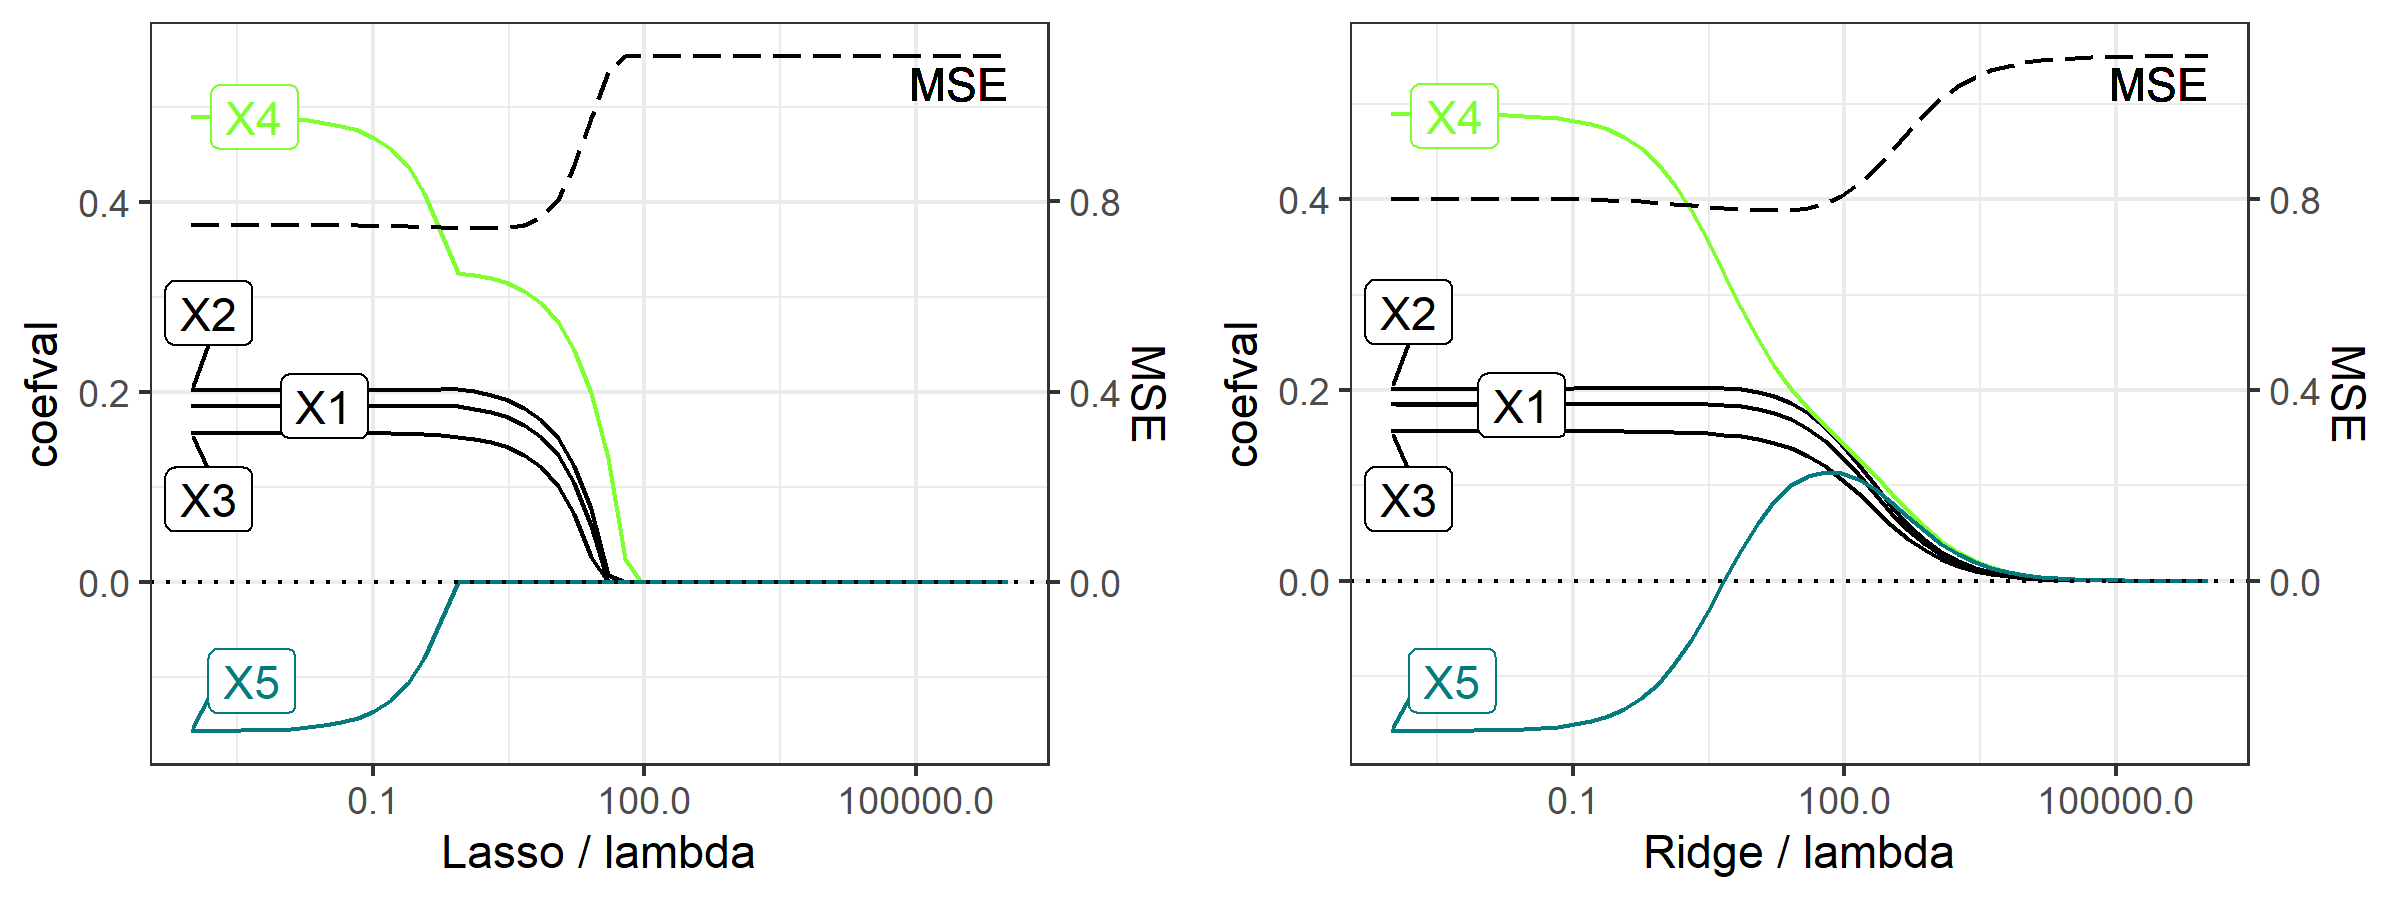
\includegraphics[width=0.65\textwidth]{sl/feature-selection/figure/regu_example_lasso_ridge.png}
%\footnotesize{Lasso vs ridge regularization.}
\end{center}


\end{vbframe}





\section{Filtering}


% \includepdf[pages={2},trim=0 20 0 0,clip,width=490pt,offset=-10pt 10pt,pagecommand={}]{sl/slides-fs-filters1.pdf} 
% pages 2, 4, 5, 7

\begin{frame2}{Introduction}
  \vspace{0.4cm}
  \begin{itemize}
  \setlength{\itemsep}{0.8em}
    \item \textbf{Filter methods} construct a measure that quantifies the dependency between features and the target variable
    \item They yield a numerical score for each feature $x_j$, according to which we rank the features
    \item They are model-agnostic and can be applied generically
    %\item Filter methods are strongly related to methods for determining variable importance.
  \end{itemize}
  \vspace{-0.2cm}
  \begin{center}
  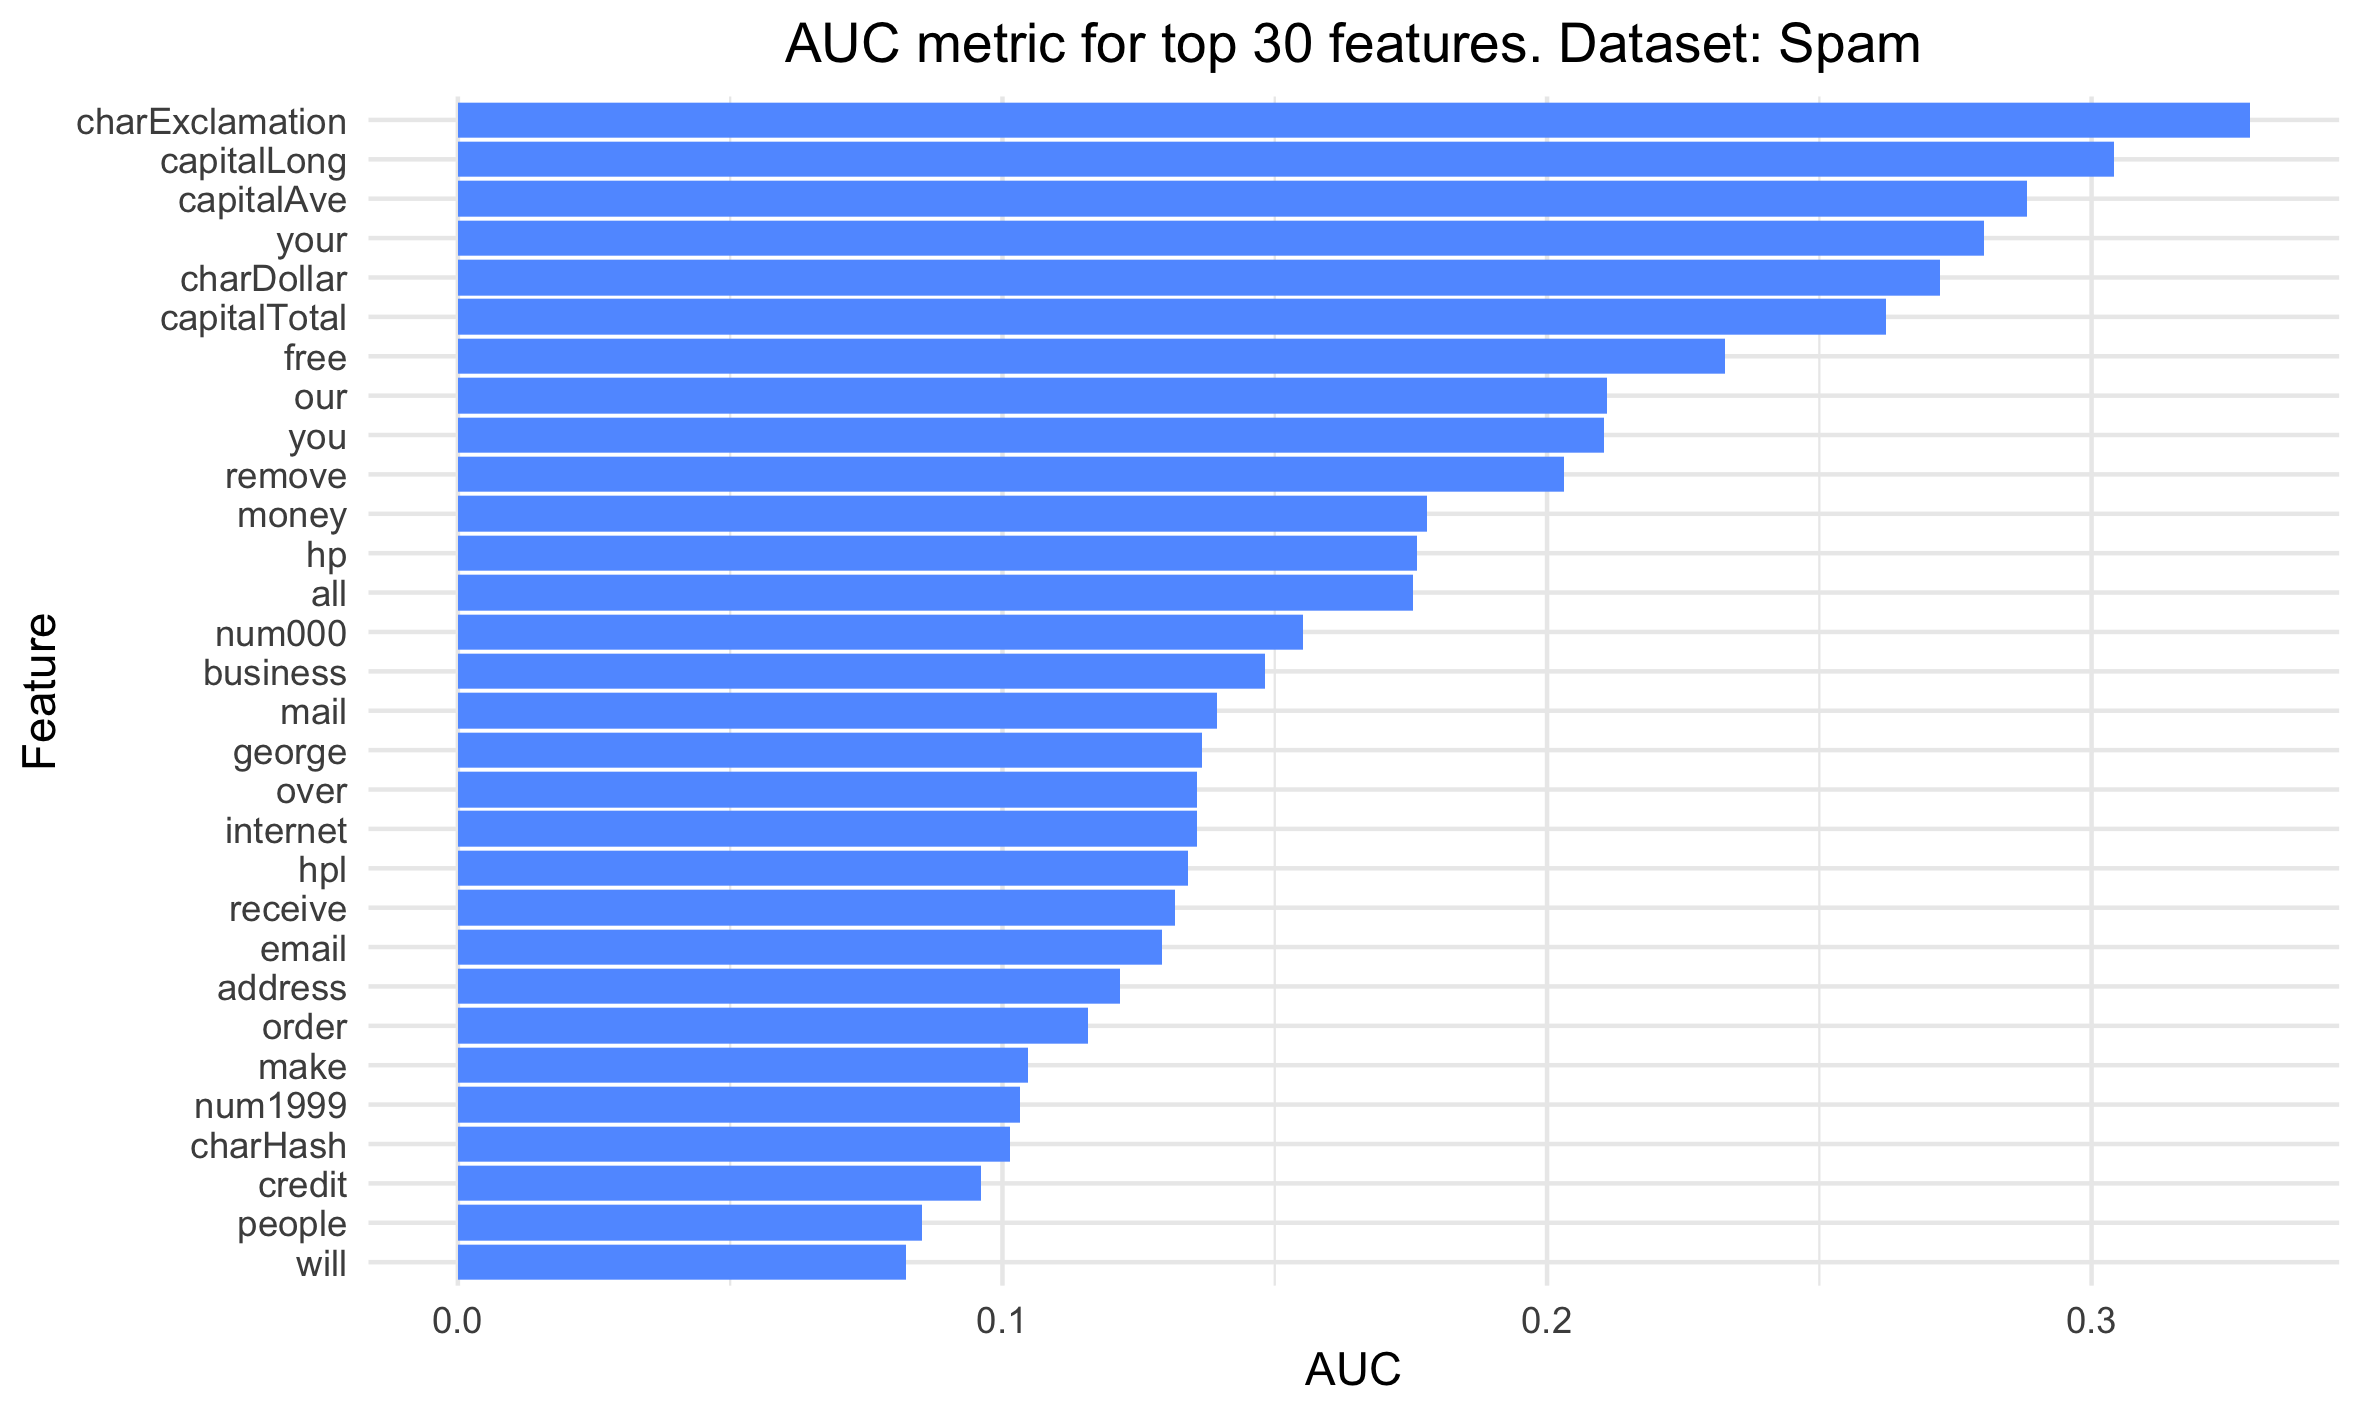
\includegraphics[width=0.55\textwidth]{sl/feature-selection/figure/fs-auc-barplot.png}\\
  \footnotesize{Exemplary filter score ranking for Spam data}
  \end{center}
  
\end{frame2}

% 4, 5

\begin{frame2}{Pearson \& Spearman correlation}
\textbf{Pearson correlation $r(x_j, y)$: }
\begin{itemize}
\item For numeric features and targets only
\item Measures linear dependency
\item $ r(x_j, y) = \frac{\sum_{i=1}^n (x^{(i)}_j - \bar{x}_j) (\yi - \bar{y})}{\sqrt{\sum_{i=1}^n (x^{(i)}_j - \bar{x}_j)} \sqrt{(\sum_{i=1}^n \yi - \bar{y})}},\qquad -1 \le r \le 1$
\end{itemize}
\vspace{0.4cm}
\textbf{Spearman correlation $r_{SP}(x_j, y)$:}
\begin{itemize}
\item For features and targets at least on ordinal scale
\item Equivalent to Pearson correlation computed on ranks
\item Assesses monotonicity of relationship
% \item Calculate the Spearman correlation coefficient between each feature-target combination:
% $$ r_{SP} = \frac{\sum (rg(\xi) - \bar{rg}_x) (rg(\yi) - \bar{rg}_y)}{\sqrt{\sum (rg(\xi) - \bar{rg}_x)^2 \sum (rg(\yi) - \bar{rg}_y)^2}}$$
% $-1 \le r_{SP} \le 1$
% 
% $r_{SP} > 0$: positive correlation.
% 
% $r_{SP} < 0$: negative correlation.
% 
% $r_{SP} = 0$: no correlation.
% \item A higher score indicates a higher relevance of the feature.
\end{itemize}
\lz
Use absolute values $|r(x_j, y)|$ for feature ranking:\\
higher score indicates a higher relevance

\end{frame2}
\begin{frame2}{Pearson \& Spearman correlation}

Only \textbf{linear} dependency structure, non-linear (non-monotonic) aspects are not captured:

\lz

% in rsrc/chunk2_filter_correlation.R created
\begin{center}
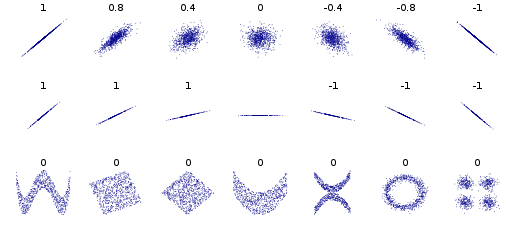
\includegraphics[width=0.75\textwidth]{sl/feature-selection/figure_man/correlation_example.png}\\
\footnotesize{Comparison of Pearson correlation for different dependency structures.}
\end{center}
%Comparison of Pearson correlation for different dependency structures.\\
\vspace{0.1cm}
To assess strength of non-linear/non-monotonic dependencies, generalizations such as \textbf{distance correlation} can be used.

% \begin{center}
%   
\includegraphics[width=0.9\textwidth]{figure_man/correlation_example.png}
% 
%   \scriptsize{\url{https://en.wikipedia.org/wiki/Pearson\_correlation\_coefficient\#/media/File:Correlation\_examples2.svg}}
% \end{center}
% 
% \begin{vbframe}{Filter: Rank correlation}
% \begin{itemize}
%   \item For features and targets at least on ordinal scale.
%   \item Equivalent to Pearson correlation computed on the ranks.
%   \item Assesses monotonicity of the dependency relationship.
% \item Calculate the Spearman correlation coefficient between each feature-target combination:
% $$ r_{SP} = \frac{\sum (rg(\xi) - \bar{rg}_x) (rg(\yi) - \bar{rg}_y)}{\sqrt{\sum (rg(\xi) - \bar{rg}_x)^2 \sum (rg(\yi) - \bar{rg}_y)^2}}$$
% $-1 \le r_{SP} \le 1$
% 
% $r_{SP} > 0$: positive correlation.
% 
% $r_{SP} < 0$: negative correlation.
% 
% $r_{SP} = 0$: no correlation.
% \item A higher score indicates higher relevance of the feature.
%   \end{itemize}
% \end{vbframe}
\end{frame2}


% 7
\begin{frame2}{AUC/ROC}
\begin{itemize}
\item For binary classification with $\Yspace = \{ 0, 1\}$ and numeric features
\item Classify samples using single feature (with thresholds), compute AUC per feature as proxy for its ability to separate classes 
%\item Uses each feature's values to classify samples for different thresholds, computing AUC per feature as proxy for its ability to separate classes.
\item Features are then ranked; higher AUC scores $\to$ higher relevance.
\end{itemize}
%Text explaining the AUC feature selection method here (calculate ROC curve thresholded on each individual feature, larger the better,...)
\begin{center}
\begin{figure}
    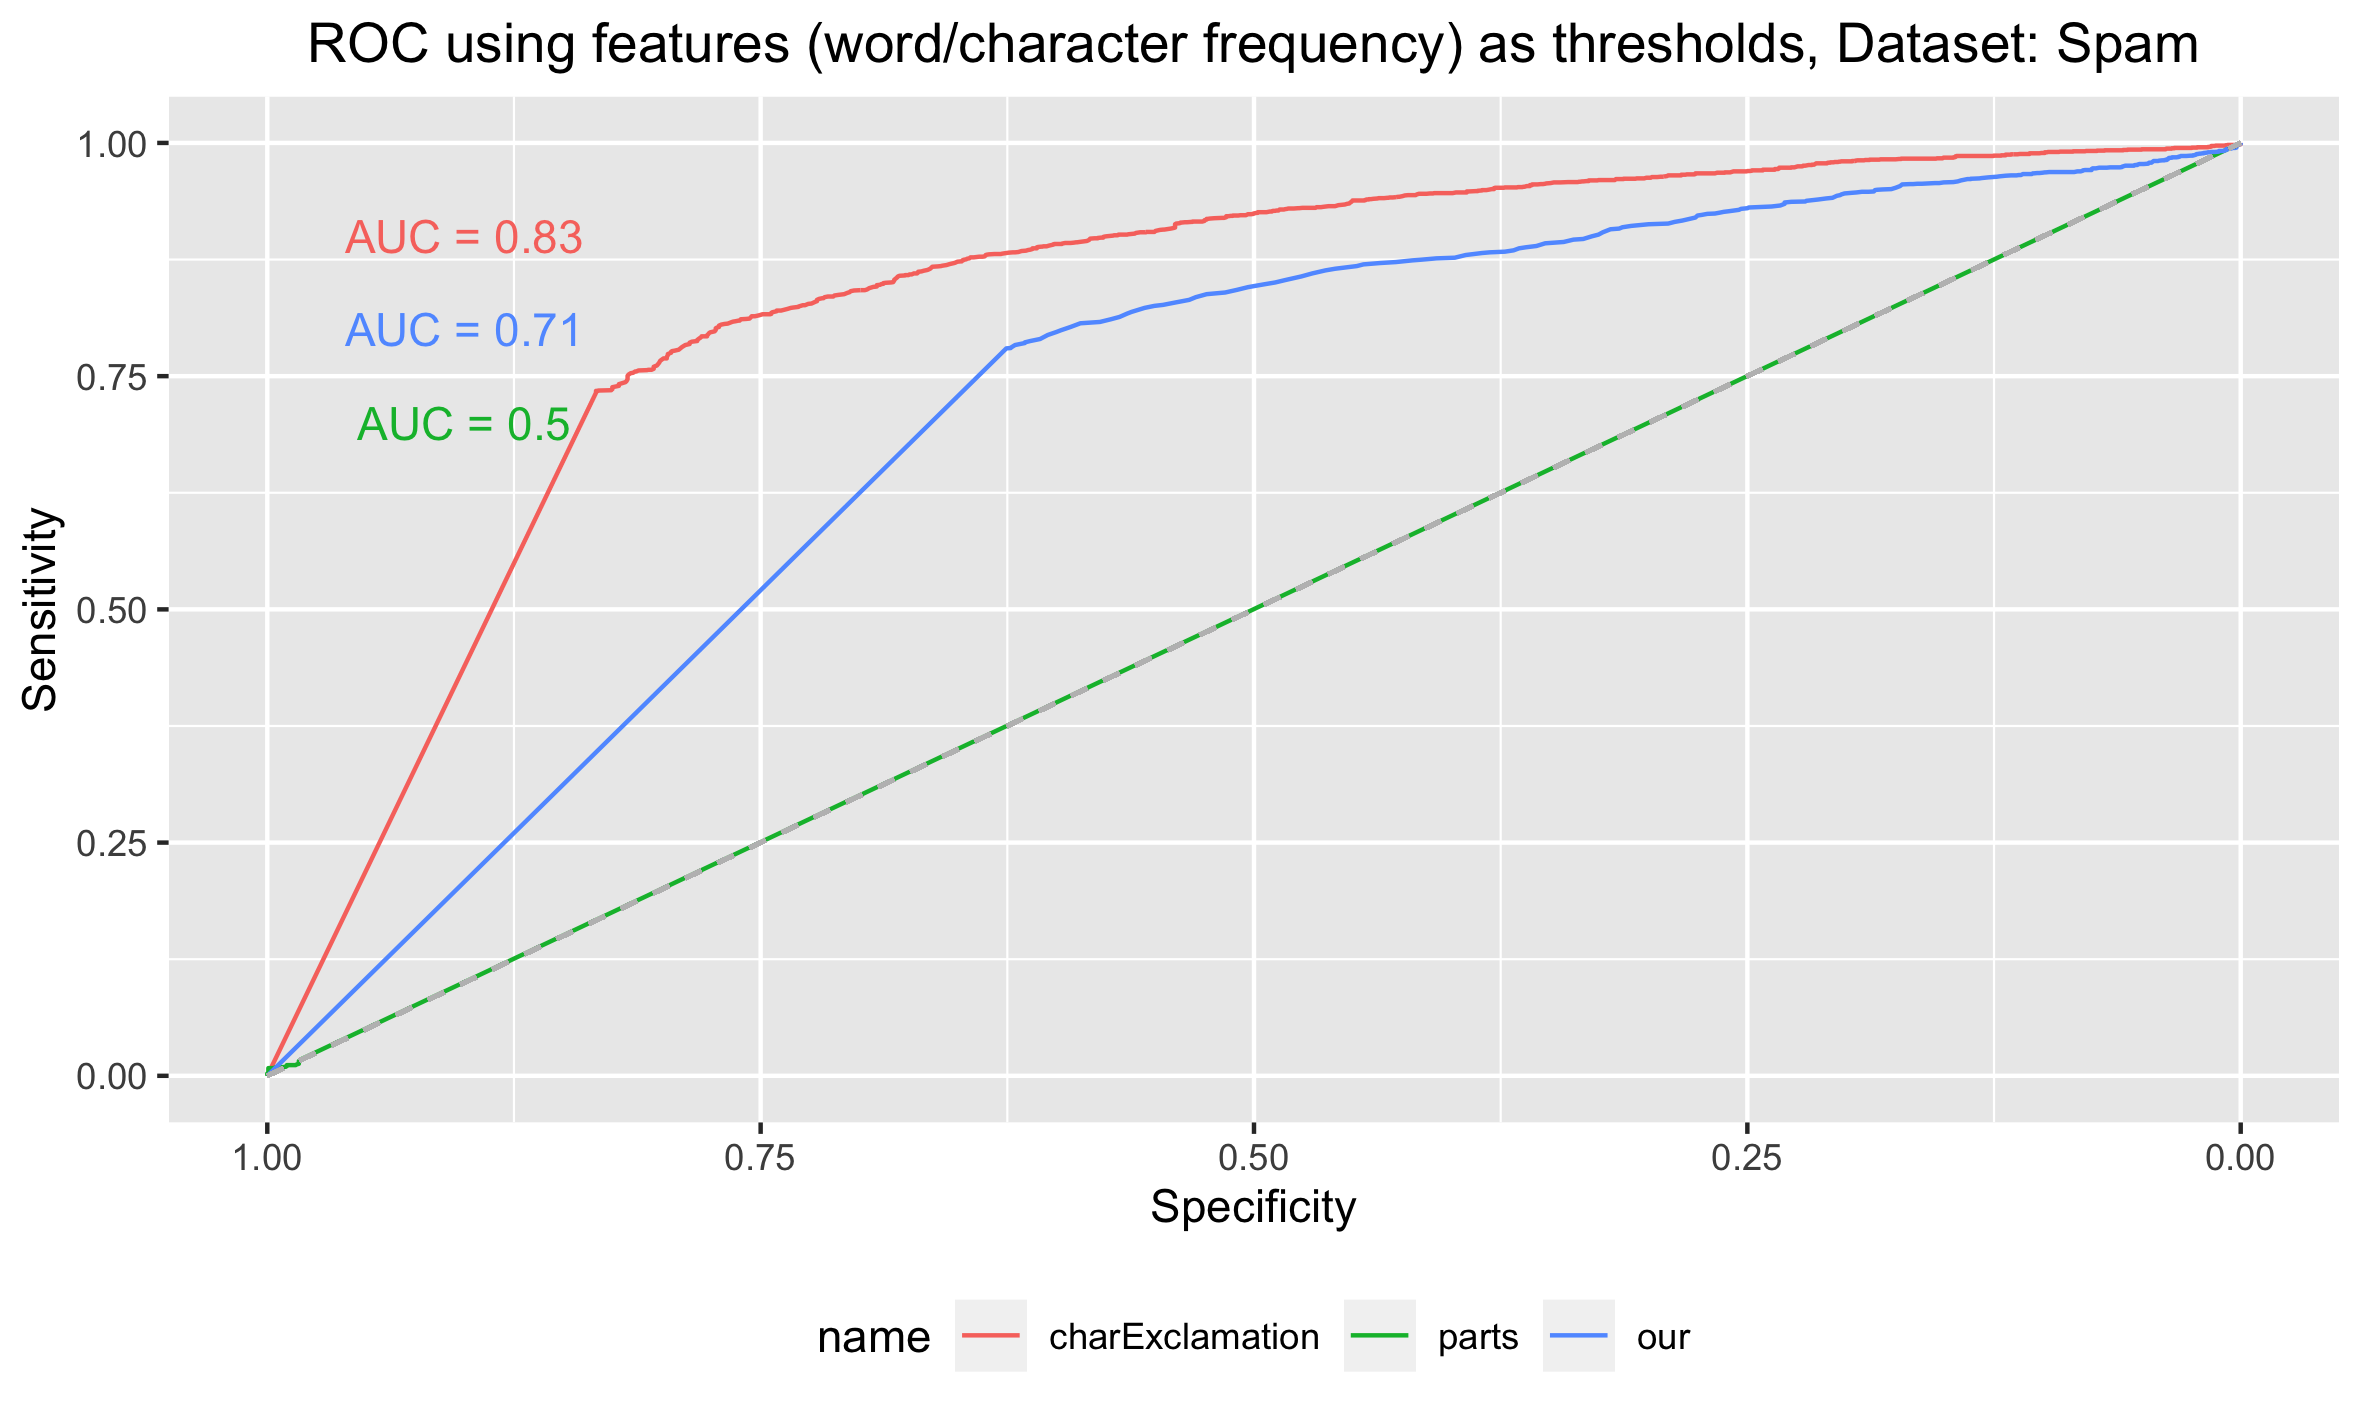
\includegraphics[width=0.7\textwidth]{sl/feature-selection/figure/fs-roc-curve.png}
\end{figure}

%\footnotesize{Isabelle Guyon, André Elisseeff (2003). An Introduction to Variable and Feature Selection.  Journal of Machine Learning Research (3) p. 1157-1182.}
\end{center}
\end{frame2}




\begin{frame}{Further Criteria/Methods}
    \begin{itemize}
        \item Classification
        \begin{itemize}
            \item $\chi^2$-statistic
            \item Welch's t-Test
            \item F-Test
            
        \end{itemize}
        \item Regression \& Classification
        \begin{itemize}
            \item Mutual Information
            \item Relief
        \end{itemize}
        \item Model-based
        \begin{itemize}
            \item Tree-based feature importance (decision tree, extra trees, random forest)
            \item Coefficients of linear model
        \end{itemize}
    \end{itemize}
\end{frame}

% \includepdf[pages={5},trim=0 20 0 0,clip,width=490pt,offset=0pt 10pt,pagecommand={}]{sl/slides-fs-filters2.pdf} 
\begin{vbframe}{Using Filter Methods}

% \begin{minipage}{0.45\textwidth}
%     \centering
%     
\includegraphics[width=\textwidth]{figure/guyon_example_xor.png} % second figure itself
%     %\caption{second figure}
% \end{minipage}

\begin{columns}
\begin{column}{0.65\textwidth}
    \begin{enumerate}{}
    \setlength{\itemsep}{1.2em}
        \item Calculate filter score for each feature $x_j$
        \item Rank features according to score values
        \item Choose $\tilde{p}$ best features
        \item Train model on $\tilde{p}$ best features
    \end{enumerate}

    \begin{blocki}{How to choose $\tilde{p}$?}
        \item Could be prescribed by application
        \item Eyeball estimation: read from filter plots
        \item Treat as hyperparameter and tune in a pipeline, based on resampling
    \end{blocki}
\end{column}

\begin{column}{0.46\textwidth}
    %\vspace{1cm}
    \begin{figure}
    \centering
    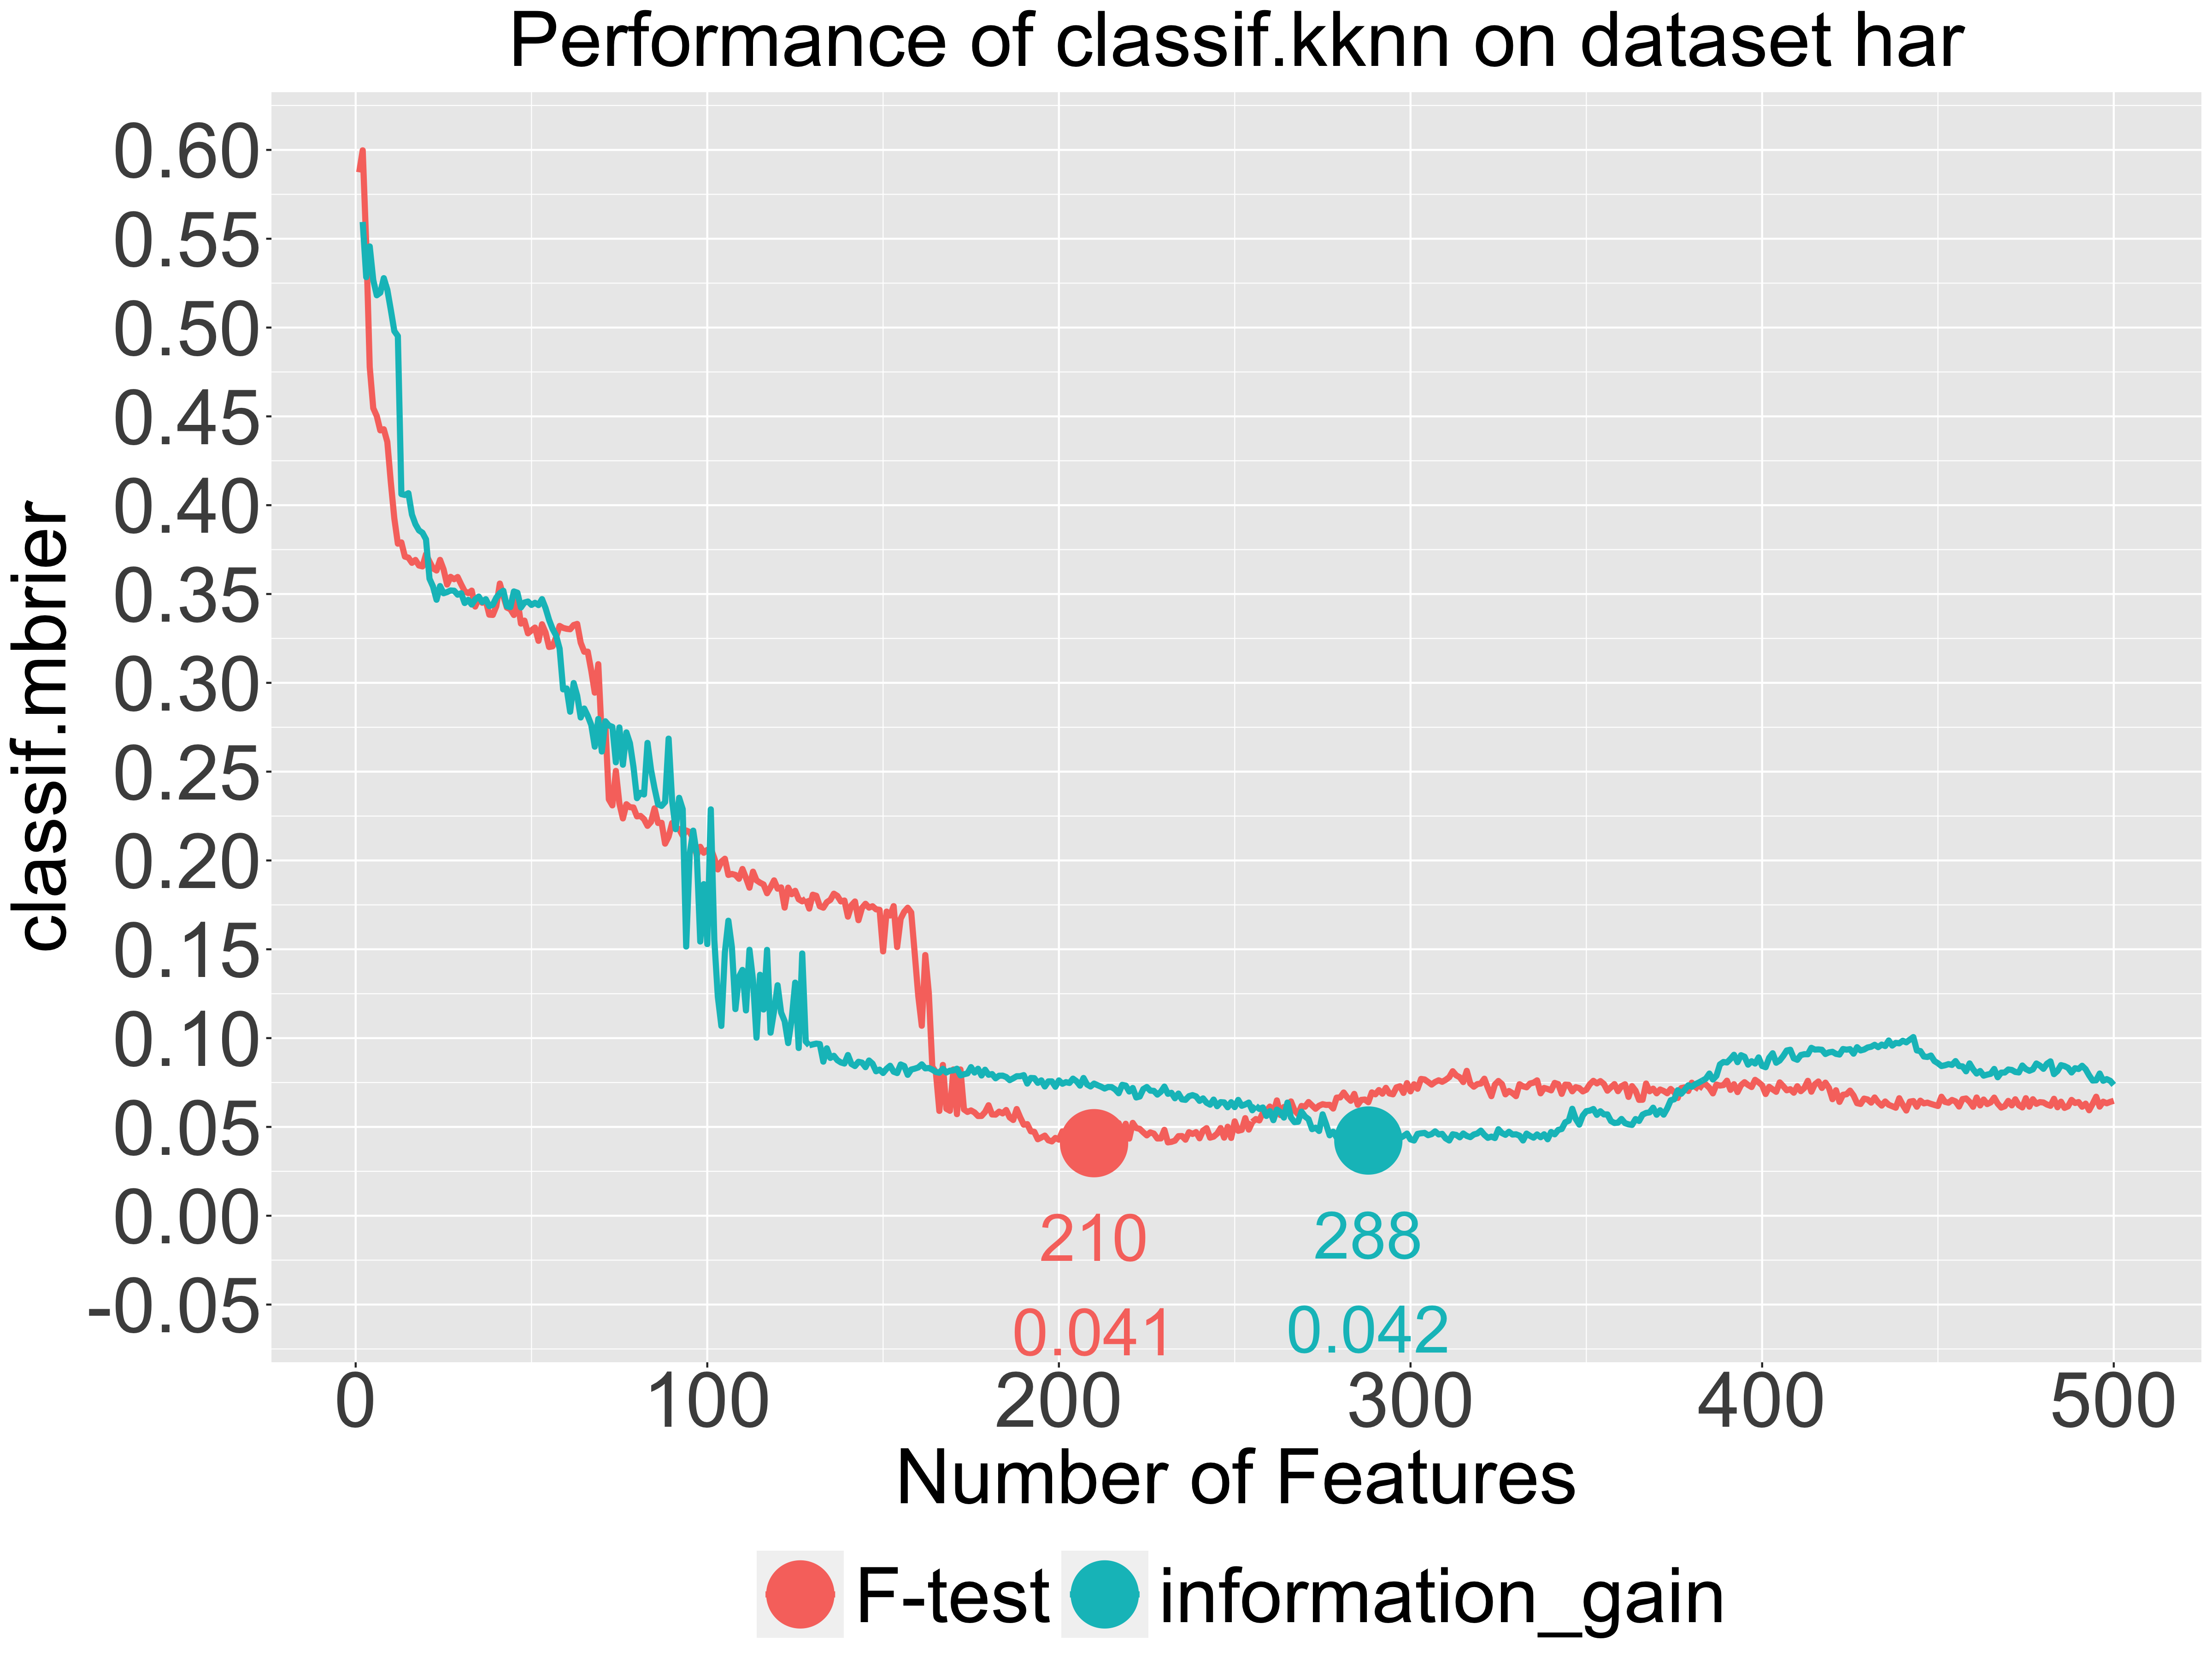
\includegraphics[width=0.89\textwidth]{sl/feature-selection/figure/filter_comparison_har_classif.kknn.png}
    \end{figure}
    \vspace{-0.4cm}
    \begin{figure}
    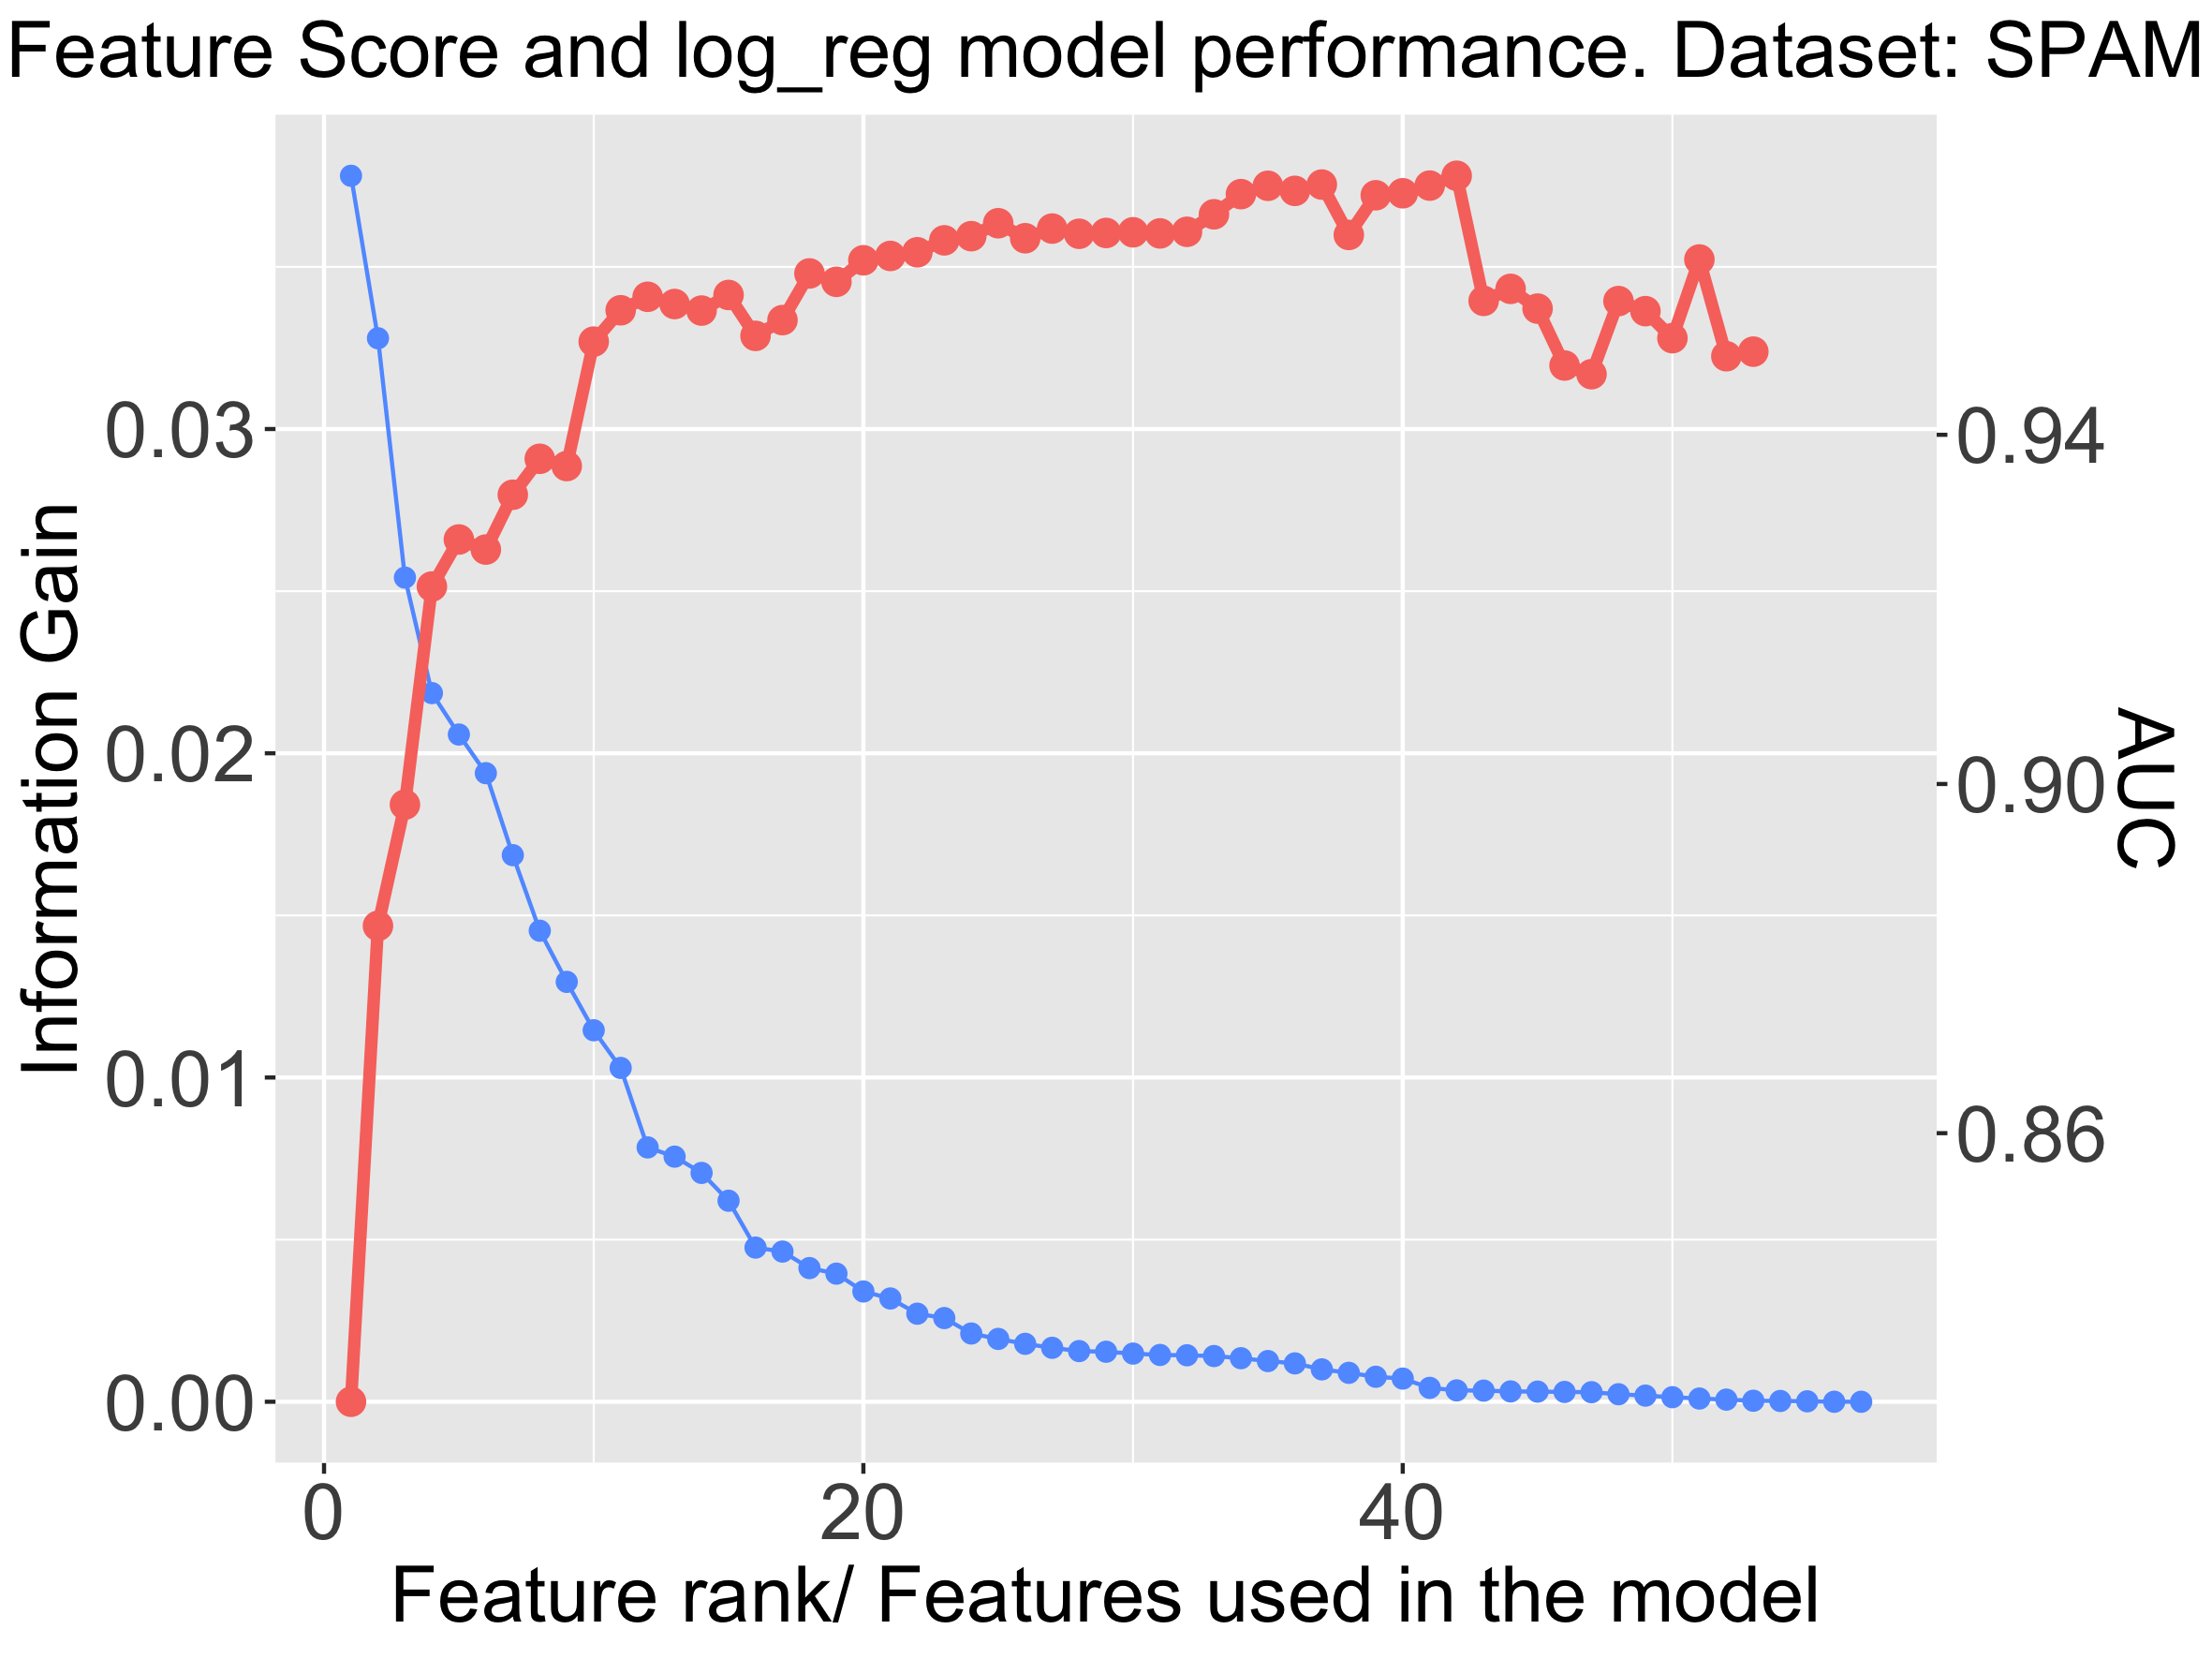
\includegraphics[width=0.89\textwidth]{sl/feature-selection/figure/fs-filters-scree-plot.png}
    \end{figure}
\end{column}

\end{columns}
\end{vbframe}

\begin{vbframe}{Advantages and Disadvantages}
    Advantages
    \begin{itemize}
        \item Fast
        \item Typically scales well with the number of features $p$
        \item Generally interpretable
        \item Can be used with any inducer
    \end{itemize}
    Negative
    \begin{itemize}
        \item Does not take specifics of the inducing algorithm into account
        \item Redundant features will have similar weights
        \item Often univariate
    \end{itemize}
\end{vbframe}

\section{Wrapper}

% for pages 5-9
% Find GFS visualization here: https://github.com/slds-lmu/lecture_sl/blob/f449ededa986978ceeb8e3a36d4ffc69ed8c7476/slides/feature-selection/rscr/fs-wrappers-visualization.R#L163


% \includepdf[pages={2},trim=0 20 0 0,clip,width=490pt,offset=0pt 10pt,pagecommand={}]{sl/slides-fs-wrapper.pdf} 
% 2-9
\begin{vbframe}{Introduction}

    \begin{itemize}
      \item Wrapper methods emerge from the idea that different sets of features can be optimal for different learners
      %\item Use the learner itself to assess the quality of the feature sets
      %\item Evaluation on a test set or resampling techniques are used
      \item Wrapper is a discrete search strategy for $S$, where objective criterion is test error of learner as function of $S$. Criterion can also be calculated on train set, approximating test error (AIC, BIC)
    \end{itemize}
    $\Rightarrow$ Use the learner to assess the quality of the feature sets
\vspace{-0.1cm}
    \begin{center}
     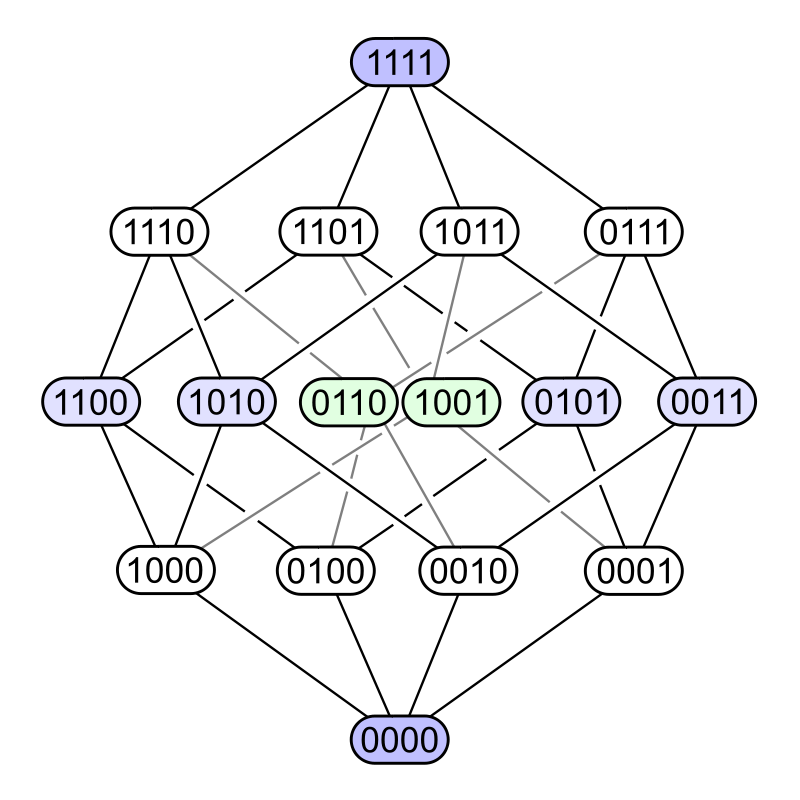
\includegraphics[width = 0.3\textwidth]{sl/feature-selection/figure/searchspace_binary.png}\\
     \scriptsize{Hasse diagram illustrating search space. Knots are connected if Hamming distance = 1 \\(Source: Wikipedia)}
    \end{center}


\end{vbframe}


% \begin{vbframe}{Introduction}

%     Wrappers have the following components:


%     \begin{itemize}
%       \item A set of starting values
%       \item Operators to create new points out of the given ones
%       \item A termination criterion
%     \end{itemize}


%     \begin{figure}
%       
\includegraphics[width=8cm]{figure_man/varsel_space.png}
%       % \caption{Space of all feature sets for 4 features.
%       % The indicated relationships between the sets insinuate a greedy search strategy which either adds or removes a feature.}
%       % Übersetzung von:
%       % Raum aller Feature-Mengen bei 4 Features. Die eingezeichnete Nachbarschaftsbeziehung unterstellt eine Art ,,gierige'' Suchstrategie, bei der wir entweder ein Feature hinzufügen oder entfernen.}
%     \end{figure}


%   \end{vbframe}

  \begin{vbframe}{Objective function}

    %\small

    Given $p$ features, \textbf{best-subset selection problem} is to find subset $S \subseteq \{ 1, \dots p \}$ optimizing objective $\Psi: \Omega \rightarrow \R$:
    \vspace{-0.15cm}
    %measuring the learner's generalization performance. The solution $S^*$ to the problem is
    $$S^{*}  \in \argmin_{{S \in \Omega}} \{ \Psi(S) \}$$
    %
    \vspace{-0.8cm}
    \begin{itemize}
    \setlength{\itemsep}{0.8em}
     \item $\Omega$  = search space of all feature subsets $S\subseteq\{ 1, \dots, p \}$. Usually we encode this by
      %(i.e., $\Omega \subseteq \mathcal{P}(\{ 1, \dots, p \})$, $\mathcal{P}$ denoting the power set)
      bit vectors, i.e., $\Omega = \{0, 1\}^p$ (1 = feat. selected)
      %It will be clear from the context which variant we refer to.
     \item Objective $\Psi$ can be different functions, e.g., AIC/BIC for LM or cross-validated performance of a learner
     \item Poses a discrete combinatorial optimization problem over search space of size = $2^p$, i.e., grows exponentially in $p$ (power set)%as it is the power set of $\{1,\ldots,p\}$
      %also known as $L_0$ regularization.
     \item Unfortunately can not be solved efficiently in general (NP hard; see, e.g., \furtherreading{NATARAJAN1995SPARSE})
     \item Can avoid searching entire space by employing efficient search strategies, traversing search space in a ``smart" way %that finds performant feature subsets

    \end{itemize}

  \end{vbframe}


%  \begin{vbframe}{How difficult is best-subset selection?}

%     \begin{itemize}
%     \setlength{\itemsep}{1em}
%       \item Size of search space = $2^p$, i.e., grows exponentially in $p$ as it is the power set of $\{1,\ldots,p\}$
%       \item Finding best subset is discrete combinatorial optimization problem.
%       %also known as $L_0$ regularization.
%      \item It can be shown that this problem unfortunately can not be solved efficiently in general (NP hard; see, e.g., \furtherreading{NATARAJAN1995SPARSE})
%      \item We can avoid having to search the entire space by employing efficient search strategies, moving through the search space in a smart way that finds performant feature subsets
%      %\item By employing efficient search strategories, we can avoid searching the entire space.
%     %\item Of course this does not mean that we have to search the entire space, since there are more efficient search strategies.
%     %  \item Formally spoken: One can show that the problem is NP-hard!
%     %  \item This means that the problem cannot be solved in polynomial (P) time: ${\mathcal{O}} (p^c)$, where $c \in \N$ indicates the degree o the polynom.
%     % \end{blocki}
%     %
%     % \framebreak
%     %
%     % \begin{blocki}{How difficult is it to solve the introduced optimization problem, hence, to find the optimal feature set?}
%     %  \item More precisely, the proof demonstrates that this problem cannot be approximated within any constant, unless P = NP.
%     %
%     %   The latter means, that if you find an algorithm that solves a more difficult class of problems (than this optimization problem) in polynomial time, this implies that you found how to solve all easier problems (including our optimization problem) in polynomial time.
%     % \item \textbf{Attention}: This does not imply that it is useless trying to construct strategies which work in practice!
%     %\item Thus our problem now consists of moving through the search space in a smart and efficient way, thereby finding a particularly good set of features.
%     \end{itemize}
%   \end{vbframe}

% \begin{frame}{Greedy forward search}

%     \begin{blocki}{}
%       \item Let $S \subset \{1, \dots, p \}$, where $\{1, \dots p \}$ are feature indices
%       \item Start with the empty feature set $S = \emptyset$
%       \item For a given set $S$, generate all $S_j = S \cup \{j\}$ with $j \notin S$.
%       \item Evaluate the classifier on all $S_j$ and use the best $S_j$
%       \item Iterate over this procedure
%       \item Terminate if:
%         \begin{enumerate}
%           \item the performance measure doesn't improve enough
%           \item a maximum number of features is used
%           \item a given performance value is reached
%         \end{enumerate}
%     \end{blocki}

%     \end{frame}

\begin{frame}{Greedy forward search}
Let $S \subset \{1, \dots, p \}$ be subset of feature indices.
\vspace{-0.01cm}
    \begin{enumerate}
      %\item Let $S \subset \{1, \dots, p \}$, where $\{1, \dots p \}$ are feature indices
      \item Start with the empty feature set $S = \emptyset$
      \item For a given set $S$, generate all $S_j = S \cup \{j\}$ with $j \notin S$.
      \item Evaluate the classifier on all $S_j$ and use the best $S_j$
      \end{enumerate}
    %\vspace{-0.2cm}
    \textbf{Example} GFS on a subset of bike sharing data with features windspeed, temp., humidity and feeling temp. Node value is RMSE.
    \begin{center}
    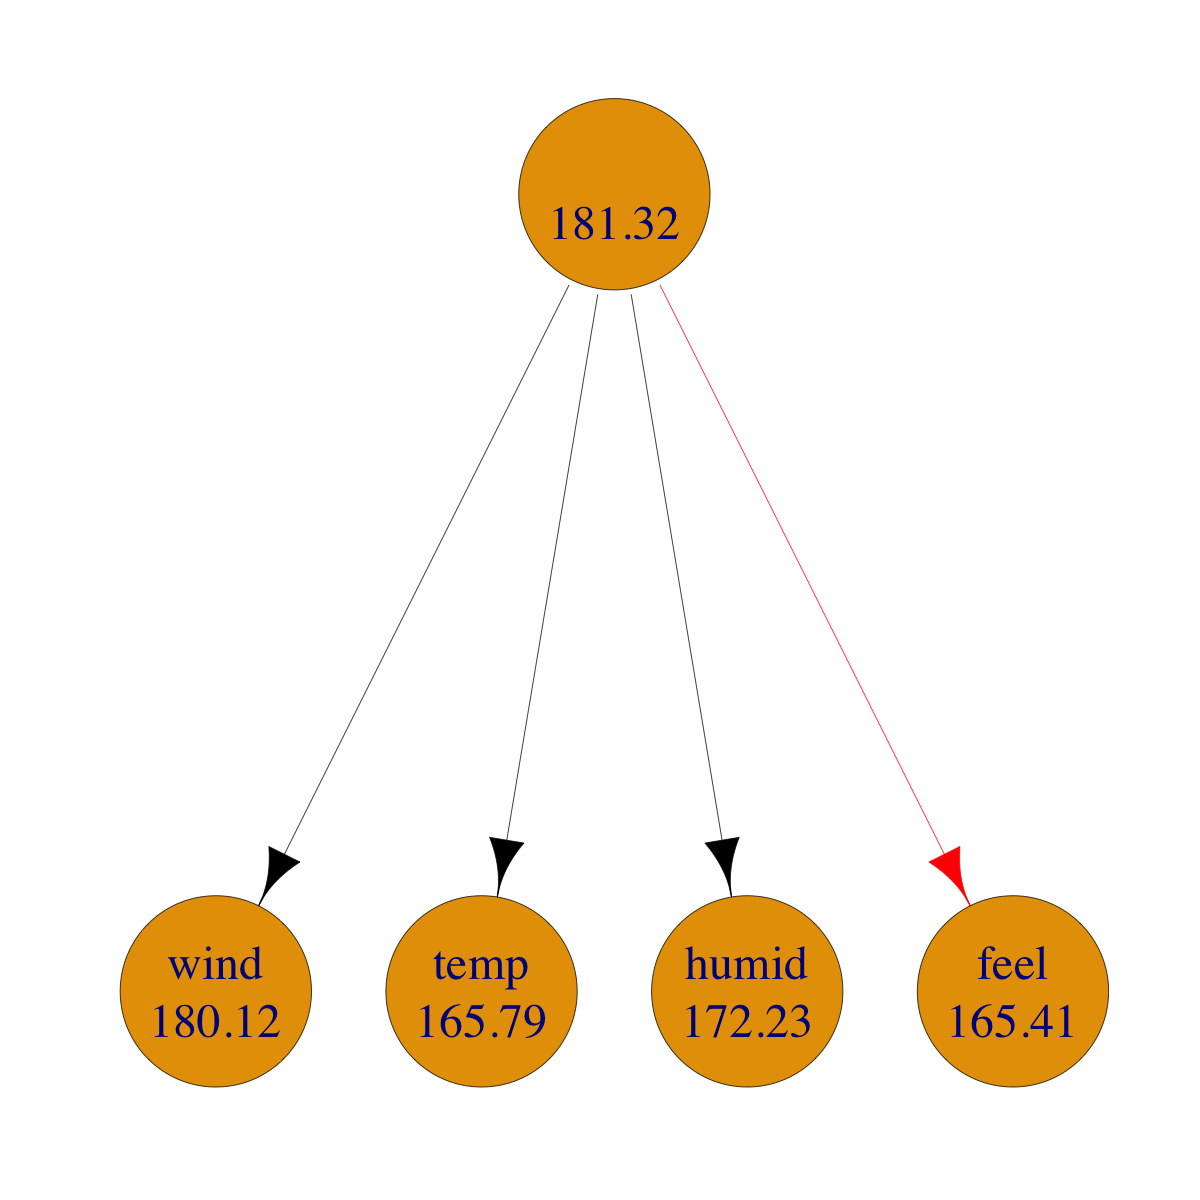
\includegraphics[width = 0.45\textwidth]{sl/feature-selection/figure/fs-wrappers-powerset-tree-1.png}
    \end{center}

\end{frame}
    %\framebreak

\begin{frame}[noframenumbering]{Visualization of GFS}
\begin{enumerate}
    \setcounter{enumi}{3}
    \item Iterate over this procedure
\end{enumerate}
    \begin{center}
      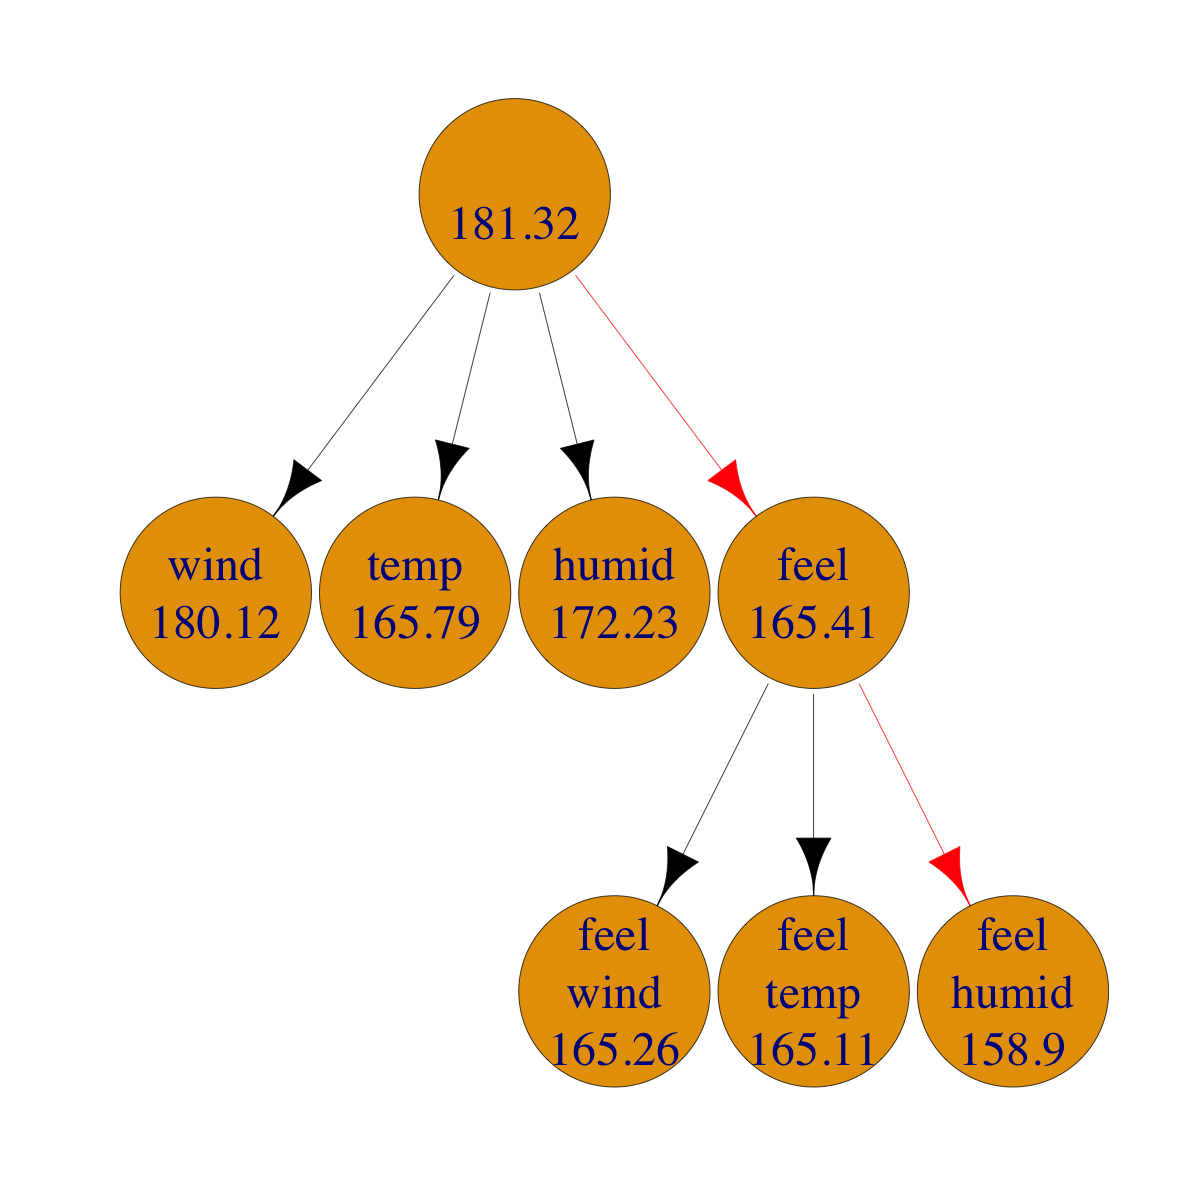
\includegraphics[width = 0.65\textwidth]{sl/feature-selection/figure/fs-wrappers-powerset-tree-2.png}
      \end{center}
      %\framebreak
\end{frame}

\begin{frame}[noframenumbering]{Visualization of GFS}
\begin{enumerate}
    \setcounter{enumi}{3}
    \item Iterate over this procedure
\end{enumerate}

    \begin{center}
      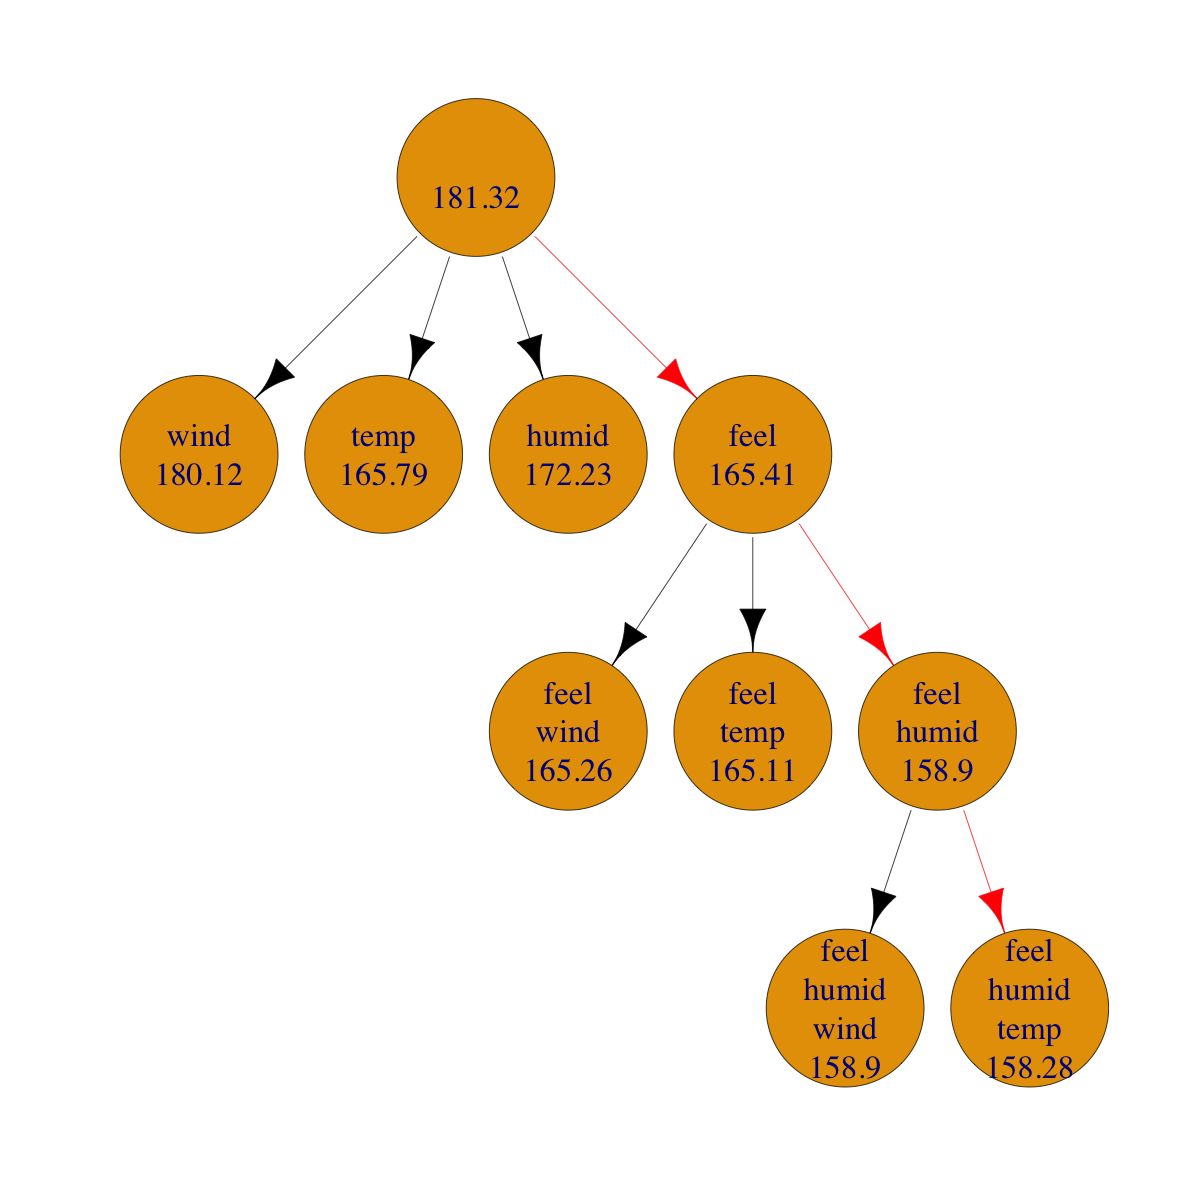
\includegraphics[width = 0.65\textwidth]{sl/feature-selection/figure/fs-wrappers-powerset-tree-3.png}
    \end{center}
\end{frame}

\begin{frame}[noframenumbering]{Visualization of GFS}
    \begin{center}
      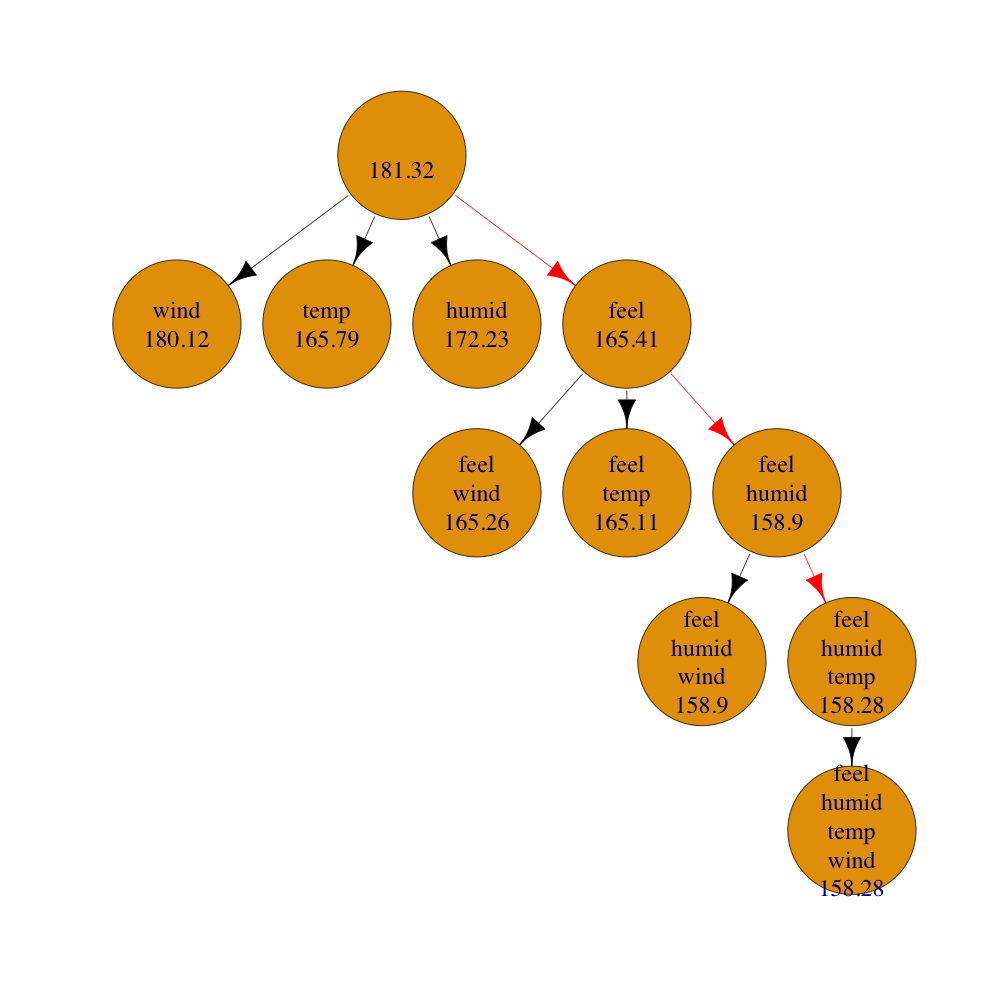
\includegraphics[width = 0.6\textwidth]{sl/feature-selection/figure/fs-wrappers-powerset-tree-4.png}
      \end{center}
      \vspace{-0.2cm}
 \begin{enumerate}
     \setcounter{enumi}{4}
     \item Terminate if performance does not improve further or max. number of features is used
 \end{enumerate}
\end{frame}

%\begin{frame}[noframenumbering]{Visualization of GFS}
%    \begin{center}
%    
\includegraphics[width = 0.65\textwidth]{figure/fs-wrappers-powerset-all-4.png}
%    \end{center}
%  \end{frame}


\begin{vbframe}{Greedy backward search}

    \begin{blocki}{}
      \item Start with the full index set of features $S = \{1, \ldots, p\}$.
      \item For a given set $S$ generate all

      $S_j = S \setminus\{j\}$ with $j \in S$.
      \item Evaluate the classifier on all $S_j$\
        and use the best $S_j$.
      \item Iterate over this procedure.
      \item Terminate if:
        \begin{itemize}
          \item the performance drops drastically, or
          \item falls below given threshold.
        \end{itemize}
      \end{blocki}

      \begin{itemize}
          \item GFS is much faster and generates sparser feature selections
          \item GBS much more costly and slower, but sometimes slightly better.
      \end{itemize}

  \end{vbframe}

  \begin{frame}{Visualization of GBS}
    %\begin{enumerate}
    %\setcounter{enumi}{3}
    %\item Iterate over this procedure
    %\end{enumerate}
    \textbf{Example} Greedy Backward Search on bike sharing data
    \begin{center}
      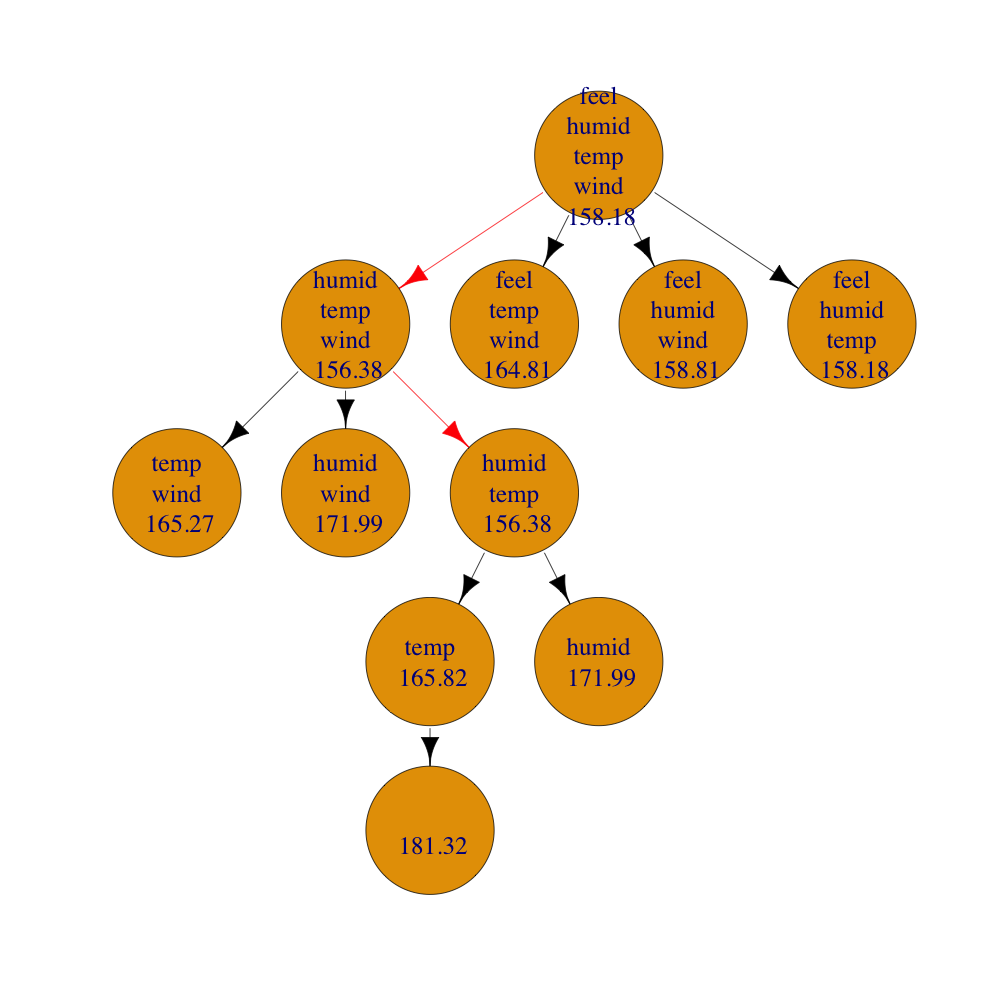
\includegraphics[width = 0.65\textwidth]{sl/feature-selection/figure/fs-wrappers-backwards-powerset-tree-4.png}
      \end{center}
      %\framebreak
\end{frame}



\begin{frame}{Advantages and Disadvantages}
    Advantages
    \begin{itemize}
        \item Inducer-agnostic
        \item Any performance measure can be used
        \item Optimizes the desired performance measure directly
    \end{itemize}
    Disadvantages
    \begin{itemize}
        \item Expensive
        \item Does not scale well with the number of features
        \item Does (in general) not use additional info about model structure
        \item Nested resampling becomes necessary
    \end{itemize}
    
\end{frame}

\section{Further Selection Techniques}

\begin{frame}{Embedded feature selection}
    \begin{itemize}
        \item Select features during the learning process
        \item Explicitly -- via regularization
        \begin{itemize}
            \item LASSO/L1
            \item Requires a solver that can set weights to zero
        \end{itemize}
        \item Implicitly -- by construction of the algorithm
        \begin{itemize}
            \item Decision-tree based algorithms
            \item Can ignore irrelevant features by not selecting them (no guarantee, though)
        \end{itemize}
    \end{itemize}
\end{frame}

% ID columns, identical columns
\begin{frame}{Domain Knowledge}
\begin{itemize}
    \item ID columns
    \begin{itemize}
        \item Often ordered, can leak time information
        \item If they identify a person etc, replace by features describing that person
        \item Contains no information that can generalize
    \end{itemize}
    \item Duplicate features
    \begin{itemize}
        \item Cause issues for (linear) models
        \item Slow down learning
        \item Reduce model interpretability
    \end{itemize}
\end{itemize}
\end{frame}

\begin{frame}{Multi-objective optimization of features}
    \begin{itemize}
        \item Optimize two competing Objectives:
        \begin{enumerate}
            \item goodness-of-fit
            \item number of variable
        \end{enumerate}
        \item Use global optimization algorithm
        \begin{itemize}
            \item Evolutionary Algorithm
            \item Sparse Bayesian optimization
        \end{itemize}
    \end{itemize}
    \begin{figure}
        \centering
        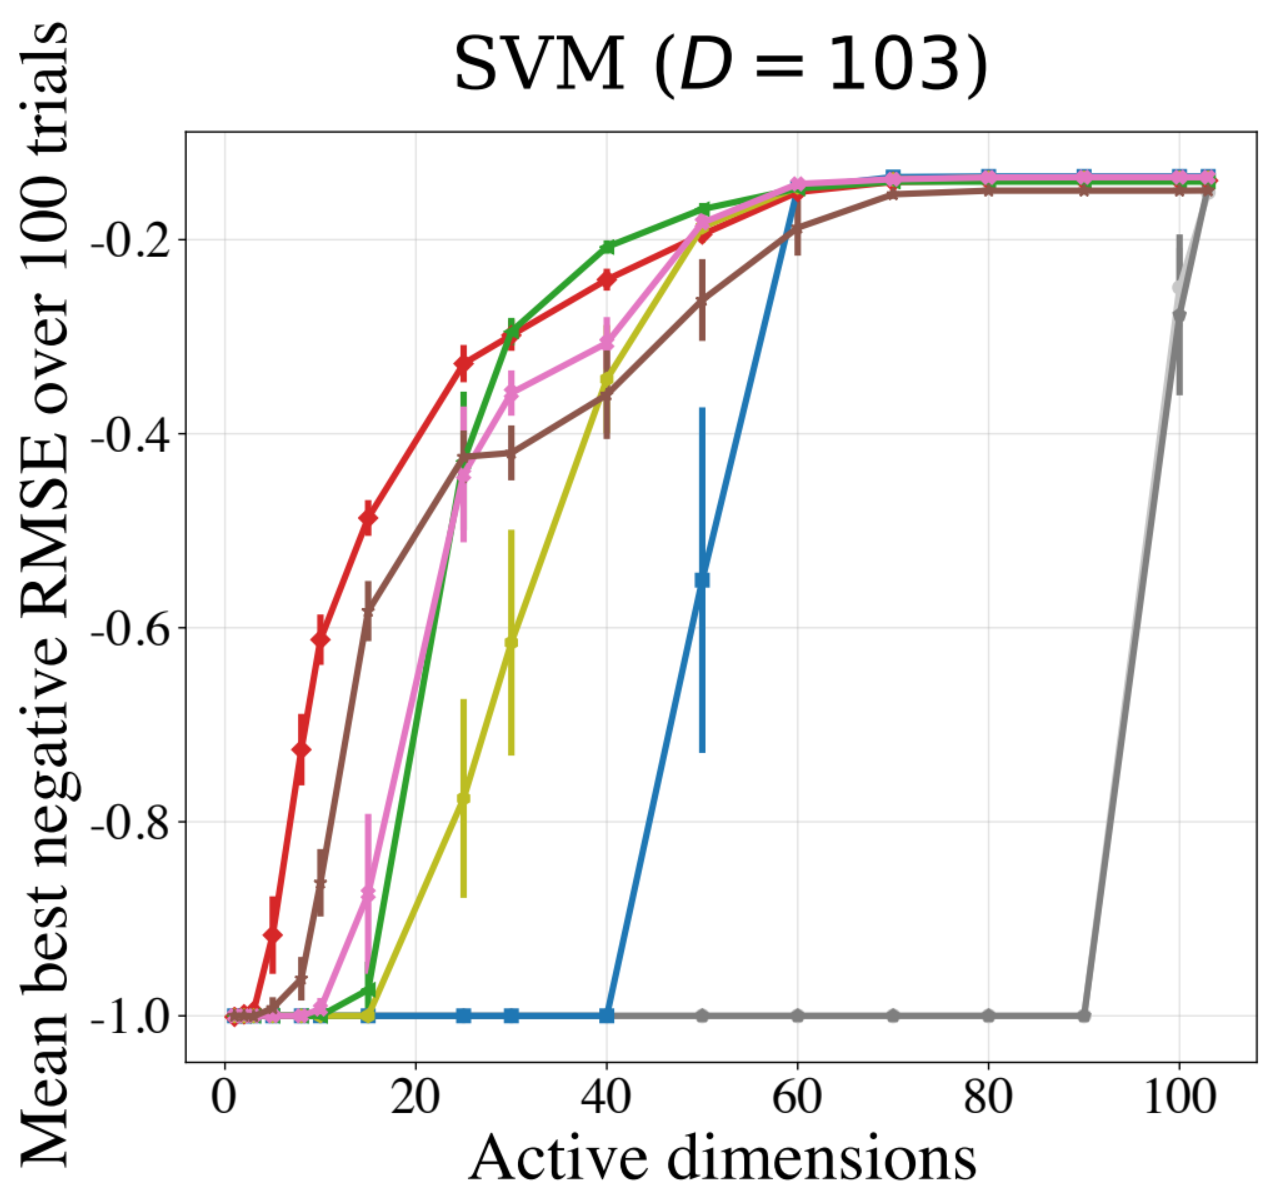
\includegraphics[width=0.4\textwidth]{figure/liu-aistats23a.png}
    \end{figure}
\end{frame}

\begin{frame}{Boruta (1)}
    \begin{itemize}
        \item All-relevant feature selection
        \newline Goal: find all features that have affect the prediction
        \newline $\rightarrow$ Can include redundant features
        \item Idea: use \emph{shadow variables} to contrast existing features against
        \item Method: Extend a feature scoring to an iterative testing mechanism
    \end{itemize}
    \vfill
    \href{https://cran.r-project.org/web/packages/Boruta/vignettes/inahurry.pdf}{Boruta for those in a Hurry by Miron B. Krusa}
\end{frame}

% TODO make pseudocode
\begin{frame}{Boruta (2)}
    \vfill
    \begin{enumerate}
        \item Create a copy of each feature, shuffle these copies
        \item Fit a random forest on the new dataset
        \item An attribute is deemed important, if its feature importance is higher than the maximal importance of all randomised attributes
        \item Repeat steps 1-3 for $N$ iterations
        \item Execute SHT with the null hypothesis that the importance of a feature is equal to the maximal importance of all randomised attributes
        \item Repeat steps 1-5 until the feature set is stable
    \end{enumerate}
    \vfill
\end{frame}

\section{Wrap-up}

\begin{frame}{Takeaways}
    \vfill
    \begin{itemize}
        \item There can be multiple goals in feature selection:
        \begin{itemize}
            \item Single Feature Selection
            \item Multiple Feature Selection
            \item All-relevant Feature Selection
        \end{itemize}
        \item Important step for good prediction quality and fast models
        \item Different feature selection methods have different goals and use different mechanisms $\rightarrow$ model selection problem
    \end{itemize}
    \vfill
\end{frame}

\endlecture
\end{document}
